\pdfoutput=1

\documentclass[11pt]{article}
\usepackage{EMNLP2023}
\usepackage{times}
\usepackage{latexsym}
\usepackage{graphicx}
\usepackage{listings}
\lstset{
  backgroundcolor=\color{gray!8},
  basicstyle=\ttfamily,
  columns=fullflexible
}
% For proper rendering and hyphenation of words containing Latin characters (including in bib files)
\usepackage[T1]{fontenc}
\usepackage[utf8]{inputenc}
\usepackage{microtype}
\usepackage{inconsolata}
\usepackage{xspace}
\usepackage{booktabs}
\usepackage{algorithm}
\usepackage{algpseudocode}
\usepackage{amsmath, amsfonts, amssymb}

\usepackage{makecell}
\usepackage[normalem]{ulem}
\usepackage{pifont}% http://ctan.org/pkg/pifont
\newcommand{\cmark}{{\ding{51}}}
\newcommand{\xmark}{{\ding{55}}}
\NewDocumentCommand{\hsb}{ mO{} }{\textcolor{pink}{\textsuperscript{\textit{Shibo}}\textsf{\textbf{\small[#1]}}}}

\NewDocumentCommand{\gy}{ mO{} }{\textcolor{purple}{\textsuperscript{\textit{Yi}}\textsf{\textbf{\small[#1]}}}}

\NewDocumentCommand{\hzt}{ mO{} }{\textcolor{red}{\textsuperscript{\textit{ZT}}\textsf{\textbf{\small[#1]}}}}

\NewDocumentCommand{\zhen}{ mO{} }{\textcolor{blue}{\textsuperscript{\textit{ZW}}\text{\text{\small[#1]}}}}

\NewDocumentCommand{\jjh}{ mO{} }{\textcolor{cyan}{\textsuperscript{\textit{Joshua}}\text{\text{\small[#1]}}}}


\newcommand{\dummyfig}[1]{
  \centering
  \fbox{
    \begin{minipage}[c][0.3\textheight][c]{0.5\textwidth}
      \centering{#1}
    \end{minipage}
  }
}

\def\blocksworld{{Blocksworld}\xspace}
\def\ours{{RAP}\xspace}

% If the title and author information does not fit in the area allocated, uncomment the following
%
%\setlength\titlebox{<dim>}
%
% and set <dim> to something 5cm or larger.

\title{Reasoning with Language Model is
Planning with World Model}

% Author information can be set in various styles:
% For several authors from the same institution:
% \author{Author 1 \and ... \and Author n \\
%         Address line \\ ... \\ Address line}
% if the names do not fit well on one line use
%         Author 1 \\ {\bf Author 2} \\ ... \\ {\bf Author n} \\
% For authors from different institutions:
% \author{Author 1 \\ Address line \\  ... \\ Address line
%         \And  ... \And
%         Author n \\ Address line \\ ... \\ Address line}
% To start a separate ``row'' of authors use \AND, as in
% \author{Author 1 \\ Address line \\  ... \\ Address line
%         \AND
%         Author 2 \\ Address line \\ ... \\ Address line \And
%         Author 3 \\ Address line \\ ... \\ Address line}

\author{%
Shibo Hao\textsuperscript{$*\clubsuit$} \ Yi Gu\thanks{\, equal contribution}\textsuperscript{$*\clubsuit$} \
Haodi Ma\textsuperscript{$\diamondsuit$}\  Joshua Jiahua Hong\textsuperscript{$\clubsuit$} \\ \textbf{Zhen Wang\textsuperscript{$\clubsuit$ $\spadesuit$} \
Daisy Zhe Wang\textsuperscript{$\diamondsuit$}\ Zhiting Hu\textsuperscript{$\clubsuit$}}  \vspace{5pt} \\
\textsuperscript{$\clubsuit$}UC San Diego, \textsuperscript{$\diamondsuit$}University of Florida\\
\textsuperscript{$\spadesuit$}Mohamed bin Zayed University of Artificial Intelligence \\
\texttt{\{s5hao, yig025, jjhong, zhw085, zhh019\}@ucsd.edu}  \\
\texttt{\{ma.haodi, daisyw\}@ufl.edu}}
 
% \author{First Author \\
%   Affiliation / Address line 1 \\
%   Affiliation / Address line 2 \\
%   Affiliation / Address line 3 \\
%   \texttt{email@domain} \\\And
%   Second Author \\
%   Affiliation / Address line 1 \\
%   Affiliation / Address line 2 \\
%   Affiliation / Address line 3 \\
%   \texttt{email@domain} \\}

\begin{document}
\maketitle
\begin{abstract}
Large language models (LLMs) have shown remarkable reasoning capabilities, particularly with chain-of-thought (CoT) prompting. However, LLMs sometimes still struggle with problems that are easy for humans, such as generating action plans to achieve given goals in an environment, or performing complex math or logical reasoning. The deficiency stems from the key fact that LLMs lack an internal \emph{world model} to predict the world \emph{state} (e.g., environment status, intermediate variable values) and simulate long-term outcomes of actions. This prevents LLMs from performing deliberate planning akin to human brains, which involves exploring alternative reasoning paths, anticipating future states and rewards, and iteratively refining existing reasoning steps. To overcome the limitations, we propose a new LLM reasoning framework, {\bf \underline{R}easoning vi\underline{a} \underline{P}lanning (RAP)}. RAP repurposes the LLM as both a world model and a reasoning agent, and incorporates a principled planning algorithm based on Monte Carlo Tree Search for strategic exploration in the vast reasoning space. During reasoning, the LLM (as agent) incrementally builds a reasoning tree under the guidance of the LLM (as world model) and rewards, and efficiently obtains a high-reward reasoning path with a proper balance between exploration \emph{vs.} exploitation. 
% As a general reasoning framework, 
We apply RAP to various challenging reasoning problems including plan generation, math reasoning, and logical inference, and demonstrate its superiority over strong baselines. RAP with LLaMA-33B even surpasses CoT with GPT-4, achieving 33\% relative improvement in a plan generation setting.\footnote{The code is available at \url{https://github.com/Ber666/llm-reasoners}}
\end{abstract}
\section{Introduction}

\begin{figure*}[!t]
    \centering
    %\vspace{-10pt}
    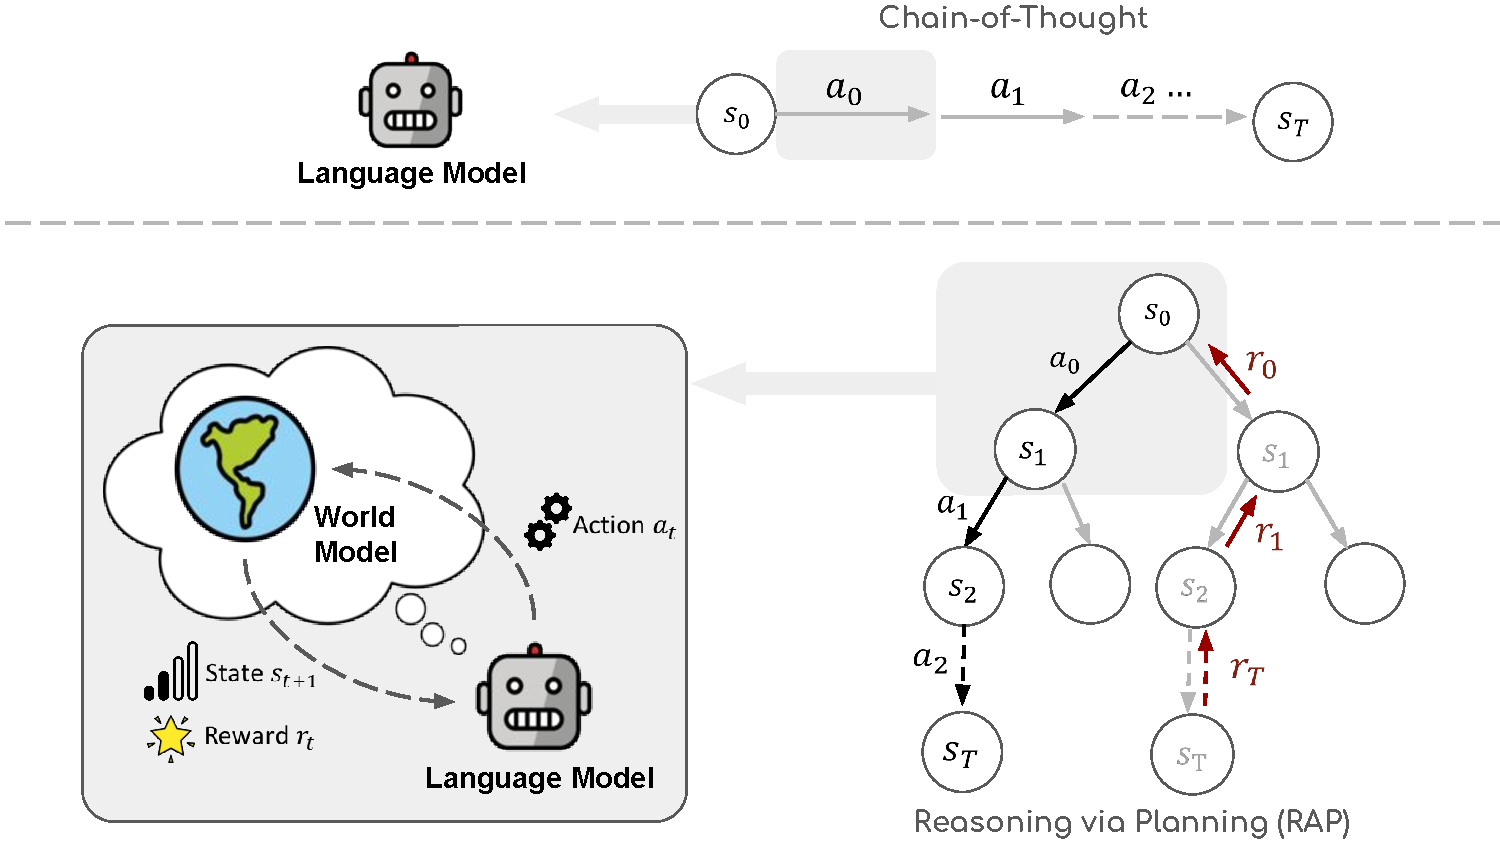
\includegraphics[width=0.8\textwidth]{sections/Figure-1_final.pdf}
    %FIGURE 1
    \vspace{-8pt}
    \caption{An overview of Reasoning via Planning (RAP). Compared with previous LLM reasoning methods like Chain-of-Thought \cite{wei2022chain}, we explicitly model the world state from a world model (repurposed from the language model), and leverage advanced planning algorithms to solve the reasoning problems.
    }
    \label{fig:1}
    \vspace{-12pt}
\end{figure*}


Large language models (LLMs) have exhibited emergent reasoning abilities in a wide range of tasks~\cite{brown2020language, chowdhery2022palm, openai2023gpt4}. Recent approaches further boost their ability by prompting LLMs to generate intermediate reasoning steps, e.g., Chain-of-Thought, CoT \cite{wei2022chain} or answer a series of subquestions, e.g., least-to-most prompting \cite{zhou2022least}. However, LLMs still face difficulties with tasks that humans find easy. For example, in creating action plans to move blocks to a target state, GPT-3 \cite{brown2020language} achieves a success rate of only 1\%, compared to 78\% for humans \cite{valmeekam2022large}; these models also struggle with complex tasks that require multiple steps of math, logical, or commonsense reasoning~\cite{ huang2022towards, mialon2023augmented}.

Humans possess an internal {\bf world model}, a mental representation of the environment~\cite{johnson1983mental, johnson2010mental, gentner2014mental}, which enables humans to simulate actions and their effects on the world's state for deliberate {\bf planning} for complex tasks of motor control, imagery, inference, and decision making \cite{tolman1948cognitive, briscoe2011mental, schulkin2012action, lecun2022path}. For example, to make an action plan towards a goal, planning with the world model involves exploring various alternative courses of actions, assessing the likely outcomes by rolling out possible future scenarios, and iteratively refining the plan based on the assessment~\cite{huys2012bonsai, gasparski2014designology, ho2021control}. This is in stark contrast to the current LLM reasoning, which instinctively generates a reasoning trace in an autoregressive manner. In particular, we identify several key limitations of the current reasoning with LLMs, including {\bf (1)} the lack of an internal world model to simulate the \emph{state} of the world (e.g., the configuration of blocks, the values of intermediate variables),
%~\cite{kratzer2007situations, zwaan2012revisiting, li2022language}), 
which is the foundation of human planning; {\bf (2)} the absence of a \emph{reward} mechanism to assess and guide the reasoning towards the desired state; and due to both limitations, {\bf (3)} the incapability of balancing \emph{exploration vs. exploitation} to efficiently explore vast reasoning space.


To address these limitations, this paper proposes a new framework, {\bf Reasoning via Planning (RAP)}, that enables LLMs to reason in a manner close to humans' conscious planning. \ours augments the LLM with a world model, and reasons with principled planning (specifically \emph{Monte Carlo Tree Search, MCTS}) to produce high-reward reasoning traces after efficient exploration (Figure~\ref{fig:1}). Notably, we acquire the world model by repurposing the LLM itself with appropriate prompts. During the reasoning, the LLM strategically builds a reasoning tree by iteratively considering the most promising reasoning steps (\emph{actions}) and using the world model (the same, repurposed LLM) to look ahead for future outcomes. The estimated future rewards are then backpropagated to update the LLM's beliefs about the current reasoning steps, guiding it to refine the reasoning by exploring better alternatives. Our MCTS-based planning effectively maintains a proper balance between exploration (of unvisited reasoning traces) and exploitation (of the best reasoning steps identified so far). 
%\hzt{Mention Aggregation here or in the experiment paragraph?}
%Aggregation is only used once and the result is not very impressive. Maybe skip it in intro
%\hsb{Compared with two concurrent works on advanced searching algorithms over the reasoning space (Guided beam search \cite{xie2023decomposition} and Tree-of-thoughts \cite{Yao2023TreeOT}), our framework stands out as a more comprehensive solution, encompassing them as a superset while also offering distinct advantages, such as the explicit state modeling, look ahead and efficient exploration.}\hzt{This is too vague. Let's discuss}

\begin{figure*}[!t]
    \centering
    %\vspace{-5pt}
    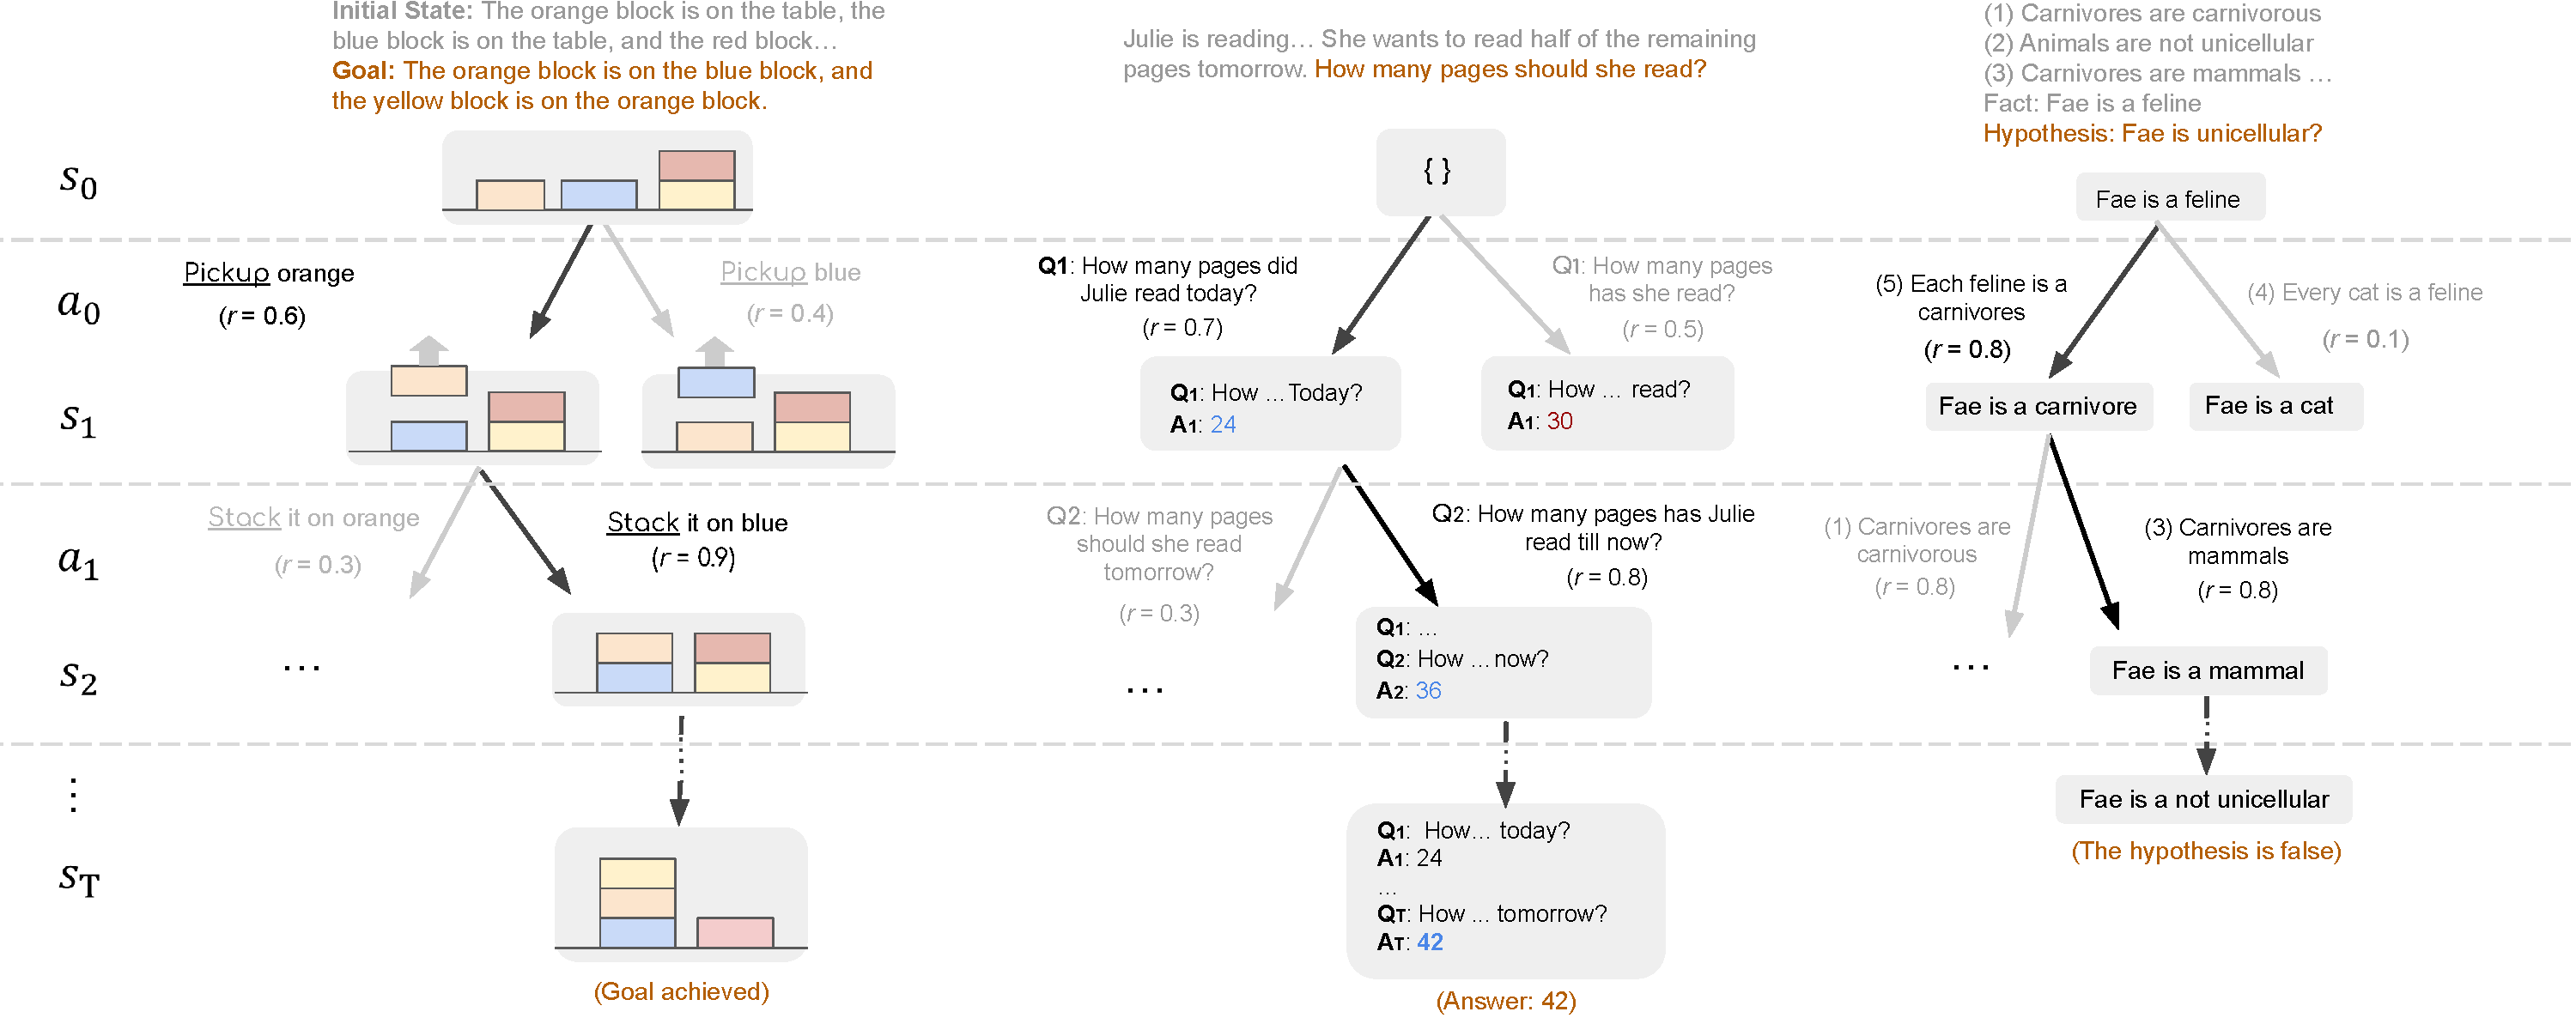
\includegraphics[width=\textwidth]{sections/Figure-2_final.pdf}
    \vspace{-22pt}
    \caption{RAP for plan generation in \blocksworld (left), math reasoning in GSM8K (middle), and logical reasoning in PrOntoQA (right).}
    \label{fig:tree_examples}
    \vspace{-15pt}
\end{figure*}

% Extensive experiments on a diverse range of challenging reasoning problems demonstrate the effectiveness of \ours by substantial improvements over various strong CoT-based reasoning approaches and even GPT-4. 
% We show that as a general reasoning framework, \ours enables a flexible formulation of rewards, states, and actions for solving distinct tasks. 
We show RAP is a general framework applicable to a diverse range of challenging problems and achieves substantial improvements over recent popular LLM reasoning methods.
For plan generation, particularly in 2/4/6-step problems of \blocksworld \cite{valmeekam2023planning}, RAP achieves an average success rate of 64\% while CoT fails almost completely. Moreover, LLaMA-33B with RAP surpasses GPT-4 with CoT by 33\% relative improvement.
In the domains of mathematical reasoning, such as GSM8K \cite{cobbe2021training} and logical inference exemplified by PrOntoQA \cite{saparov2022language}, \ours also consistently improves over strong baselines, including CoT, least-to-most prompting, and their self-consistency variants.
% beats the best CoT-based baselines by $6.8\%$ and $4.4\%$ accuracy improvement on GSM8K \cite{cobbe2021training} and PrOntoQA \cite{saparov2022language}, respectively.
 


% a diverse range of challenging problems in distinct settings, including action plan generation in a given environment , math word problems , and multi-step logical reasoning with provided logical rules (e.g., PrOntoQA \cite{saparov2022language}). RAP offers effective solutions to problems by instantiating states, actions (reasoning steps), and rewards. 
% Experiment results demonstrate substantial improvements in RAP over a range of popular reasoning approaches. On \blocksworld, \hzt{Please summarize key results}.


%\hzt{Mention previous methods as special cases?}
% maybe better mention them in the last paragraph?

% assess, roll out, 

% state, exploration/exploitation, reward/value

% plan generation (desired target state), QA (final answer)





%% ============== V1 =================


%Large language models (LLMs) \cite{brown2020language,chowdhery2022palm, touvron2023llama, openai2023gpt4} have exhibited remarkable ability across various domains, spanning abstraction, comprehension, vision, coding, mathematics, medicine, law, and understanding of human emotions \cite{bubeck2023sparks}. These exciting breakthroughs prompt researchers to consider whether these LLMs can be seen as Artificial general intelligence (AGI) \cite{bubeck2023sparks} \hzt{This paragraph is irrelevant to our work. There is no point to mention "AGI"..}. 
%However, when we compare LLMs with the human brain, it becomes apparent that current autoregressive Transformers \cite{vaswani2017attention} have an over-simplified architecture. \citet{lecun2022path} propose a conceptual architecture for AGI inspired by cognitive science and neuroscience, consisting of a configurator module, a short-term memory module, a perception module, a world model module, an actor module, and a cost module \hzt{I don't think we need to motivate ours by LeCun's paper/claims. We don't even need to mention LeCun. Perhaps fine to mention it briefly in Related Work.}. While Transformers may fit these modules implicitly during pre-training, \hzt{All the text before this point is irrelvant. We can even start the section with the following sentence.} there is evidence to suggest that current LLMs struggle with complex tasks that require the clear specification of different modules. For instance, \textbf{planning} tasks \cite{valmeekam2022large} highlight this issue \hzt{What do we mean by "planning" specifically? Need concrete examaples to articulate. Also, our work is to solve "reasoning" with the "planning" method. So "planning" is a method, not a problem to solve. Use "reasoning" to describe those problems.}.
%Until the planning is completed, an agent \gy{emphasize ``autoregressive LLM''} \hsb{Here I just want to introduce the setting of a general planning problem} is not able to interact with the real world, so it can only "guess" the results of a potential action. Additionally, a criterion is in need to evaluate and select potential actions. These two functionalities, namely the ability to predict \textbf{state transition} and to evaluate actions by providing \textbf{reward}, are primarily handled by the world model. The well-known shortage of current LLMs in planning \cite{valmeekam2022large, bubeck2023sparks} could be explained by their lack of a \textbf{world model} \cite{henaff2017model, lecun2022path, ha2018world}. \hzt{Need to introduce/motivate the concept of "world model" in a better way.}
%Given their demonstrated ability to encode rich commonsense knowledge \cite{west2021symbolic}, this failure may not be due to the ignorance of LLMs about the world,  Rather, the more plausible explanation is that the end-to-end training of LLMs doesn't encourage specialization of the world model \hzt{What does "specialization of the world model" mean?}. As such, it is worth exploring whether explicitly instructing LLMs to perform two separate roles - one as the agent and the other as the world model - results in better planning \hzt{Motivation too weak/unclear.}.



%%% ============= V2 ==============



% Large language models (LLMs) \cite{brown2020language,chowdhery2022palm, touvron2023llama, openai2023gpt4} have exhibited remarkable reasoning ability across various domains, but their ability for long-range reasoning is still very limited \cite{valmeekam2023planning} compared to humans. For example, in Blocksworld, where an agent is expected to generate an action sequence to move some blocks to a desired state, GPT-3 \cite{brown2020language} only reaches 1\% of accuracy, while humans can manage to get 78\% success rate. Given the fact that the latest LLMs reach human-level performance in many tasks, even passing a bar exam \cite{openai2023gpt4}, the failure on this commonsense task is conspicuous and prompts a question: Is long-range reasoning the Achilles' Heel of LLMs? \hsb{Keep track of state. Explain the state. Concrete examples. Reward. Guide.}

% \hsb{use the limitation as motivation. don't use other domains}
% We may get some inspiration from how people reason: Researchers in psychology and cognitive science found people use \textbf{world models} \cite{craik1967nature} that can predict the plausible state of the world. When faced with long-range reasoning task, instead of straightforwardly proposing a reasoning trace, humans may do \textbf{planning} in their mind by imagining different actions and their potential outcomes \cite{lecun2022path, kahneman2011thinking}. This procedure is also applied in optimal control \cite{bryson1975applied} and recent reinforcement learning research \cite{ha2018world}. However, most LLMs are based on autoregressive transformers and lack selective bias towards this mindset \hsb{system-2?}, which may account for their failure on reasoning tasks.

% \hsb{previous method: cot/least to most}

% In this work, we propose a novel framework to solve the reasoning via planning. We attempt to utilize the LLM as both an agent and a world model. At each reasoning step, the agent proposes some possible actions, while the world model predicts the next state and a reward. The feedback from the world model guides the agent LLM to strategically plan in two senses: (1) Given a predicted world state, it's easier for the agent LLM to propose the following actions because the remaining problem requires shorter reasoning paths (2) With the reward, we can apply Monte-Carlo Tree Search to efficiently explore and exploiting possible reasoning paths. 
% \hsb{special cases}

% \hsb{figure 1}


%While LLMs can be used as world models in classic planning problems straightforwardly, their flexibility to respond to any natural language queries enables them to address more \textbf{open} problems. Moving beyond classic planning, we explore \textbf{multi-step reasoning} by framing them as planning problems. Here, a world state is defined as a set of known variables. The agent proposes an unknown variable to reveal at each step, and then the world model reasons over its value and expands the known variable set \hzt{Unclear what do "variables" mean? What do "unknown/known" mean?}. A reward is also estimated based on its confidence and the usefulness of the reasoning step. In this context, the world model serves as an interface that encapsulates the LLM's more general understandings of the world, e.g. arithmetics and relational reasoning, rather than being limited to physical common sense.

%By formulating these planning problems within the reinforcement learning setting, we can leverage planning algorithms to solve them, such as Monte-Carlo Tree Search (MCTS). When a partial plan appears to be "promising", the agent is encouraged to revisit and continue it, while hopeless plans are discarded in favor of exploring new planning paths. 

%In the classic planning problem blockworld, our method achieves state-of-the-art performance with a substantial leap over the baseline. In multi-step reasoning problems including GSM-8k \cite{cobbe2021training} and StrategyQA \cite{geva2021did}, our method is comparable to previous sample-then-aggregate approaches like self-consistency \cite{wang2022self} with only one single path. Additionally, the human evaluation shows that our method produces more favorable paths than the baselines. \hsb{This paragraph is temporary and subject to our final results}

%In summary, we suggest using LLMs as explicit world models for planning, formulating classic planning and multi-step reasoning problems \cite{cobbe2021training, geva2021did} in an RL setting, and applying MCTS. We achieved state-of-the-art results in classic planning problems, and our proposed method outperforms previous approaches in multi-step reasoning problems. Our approach validates the need for a specialized world model to assist agents in planning, which we hope can inspire future research toward a more human-like architecture of AGI.


%We begin by focusing on \textbf{classic planning} problems, specifically represented by the blockworld \cite{valmeekam2022large}, where the agent is expected to generate an action plan to operate some blocks from an initial state to the goal state.\hsb{refer to figure 1 here} The world model serves to predict the state of the physical world so that the agent can base its future actions on the current world state. Moreover, the world model provides feedback on potential actions, such as whether they are legal or whether the new state is closer to the goal. 
%We first apply our framework to a classic plan generation task, Blockworld \cite{valmeekam2023planning}. Given a set of piles of blocks, a robot can take a sequence of actions (e.g. \textsc{stack}, \textsc{pickup}, etc.) to arrange blocks into a specified target configuration. We prompt the world model LLM to perform two jobs: (1) evaluate the action about its validity (2) describe the state of blocks given a possible action, and (3) decide whether the new state is closer to the goal state. The predicted state is appended to the prompt for agent LLM so that it can be more informed when proposing the next actions, while the rewards serve as the signals for choosing the node to expand in MCTS. 


% \vspace{-5pt}
\section{Related Work}
% \vspace{-5pt}



\noindent \textbf{Reasoning with LLMs.}
LLM reasoning typically involves decomposing complex questions into sequential intermediate steps (a.k.a. chains) before producing the final answer, exemplified by Chain-of-Thought (CoT) prompting and its variants~\cite{wei2022chain, kojima2022large}. The basic CoT generates chains all at once and can induce additional errors as the step count increases. Self-Consistency~\cite{wang2022self} samples multiple chains to choose the best answer via majority voting. Least-to-most prompting~\cite{zhou2022least} reduces the question into simpler subquestions and answers them sequentially. Similar to our reward formulation, recent works have explored self-evaluation approaches to provide feedback for intermediate steps~\cite{welleck2022generating, Shinn2023ReflexionAA, paul2023refiner}. Aligned with our state formulation, \citet{li2022language} incorporate latent ``situations'' into LLMs, referring to the state of entities from the context. More relevantly, recent works have started to explore more complex structures guided by some search algorithms. For instance, CoRe~\cite{zhu2022solving} fine-tunes reasoning step generator and verifier for math word problems with MCTS for decoding. Concurrently to our work, \citet{yao2023tree} apply heuristic-based search, like depth-/breadth-first search, for better reasoning paths. However, none of the above methods formally introduce the world model and instantiates the reward and state into a unified framework. Compared with these search-guided methods, \ours is a more principled framework to combine world model and reward with advanced planning.



%, which is designed to solve more diverse tasks. Specifically, \ours repurposes an LLM to enable flexible definitions of rewards without fine-tuning (see Section~\ref{sec:reward}), and integrates powerful search algorithms beyond heuristic search ones (see Section~\ref{sec:mcts}).

% On the other hand, exploring all possible reasoning chains or feedback can lead to scalable issues as the total number of possible chains is intractable after several steps. To tackle such issues, recent works~\cite{xie2023decomposition, Yao2023TreeOT, jung2022maieutic} use tree search to more efficiently sample possible reasoning steps. Specifically, \cite{xie2023decomposition} shares a similar decomposition strategy but in addition, follows a tree-search procedure where the LM generates multiple candidate solutions at each step toward the final problem. These candidate solutions are obtained using stochastic beam search decoding, which samples from the distribution of possible outputs. The LM then evaluates these candidates with self-evaluation, based on the quality and coherence of the generated responses. Another work similar to ours, \cite{Yao2023TreeOT}, also proposes a tree-search framework for deliberate problem-solving. The tree is constructed by considering different reasoning paths. The LLM generates and evaluates candidate paths and selects the most confident ones for further reasoning. Their approach, however, uses either depth/breadth-first search for candidate reasoning steps, while our work leverages MCTS for high-quality reward and more efficient candidate generation. CoRe\cite{zhu2022solving} introduces a cooperative reasoning framework where multiple LMs together solve math word problems. A reward model is designed to generate feedback based on the correctness of LM-generated solutions. It adopts MCTS to leverage the reward and guide the LMs to explore multiple paths for solving math problems. While their reward comes from a trained verifier, our work directly uses LLM itself to generate reward, which suits better in the zero-shot setting.

\noindent \textbf{Planning with LLMs.}
Planning, a central ability in intelligent agents, involves generating a series of actions to achieve a specific goal~\cite{mccarthy1963situations, bylander1994computational}. Classical planning methods have been widely adopted in robots and embodied environments~\cite{camacho2013model, jiang2019task}. Recently, prompting LLMs to do planning directly has gained attention and shown potential~\cite{huang2022inner, singh2022progprompt, ding2023task}. Moreover, based on LLMs' powerful programming ability~\cite{lyu2023faithful, jojic2023gpt, liu2023llm+}, recent works first translate natural language instructions into the executable programming languages, such as Planning Domain Description Language (PDDL), and runs classical planning algorithms, such as LLM+P~\cite{liu2023llm+}. However, code-based planning is constrained by its narrow domains and the environment, while \ours can handle open-domain problems, such as math and logical reasoning. More related works on \emph{world models and planning} are discussed in the Appendix~\ref{sec:related_planning}.

% \noindent \textbf{World Models and Planning.}
% Traditional reinforcement learning (RL) heavily relies on interaction with the environment (real world or simulators). To improve sample efficiency, some works leverage a \textbf{world model} that predicts state transition, and directly learn a policy within the world model \cite{ha2018recurrent, ha2018world}. With latent imagination in a world model, an RL agent can be trained to solve long-horizon tasks~\cite{hafner2019dream, hafner2020mastering}. Recent years have witnessed successful applications of \textbf{planning} algorithms in RL~\cite{sekar2020planning}, such as AlphaZero~\cite{silver2017mastering}, MuZero~\cite{schrittwieser2020mastering}. These algorithms are typically based on tree searches and are designed to effectively maintain the balance of exploration and exploitation. Compared with previous works, we use LLMs as world models and apply a planning algorithm to search for better reasoning paths, to solve various open-domain reasoning tasks.

%Daydreamer \cite{wu2023daydreamer}
% Dreamer \cite{hafner2019dream}
% Dreamer V2 \cite{hafner2020mastering}

%\cite{shyam2019model}
%Policy learning
%and DreamerV2~\cite{hafner2020mastering}
%~\cite{shyam2019model}. \cite{ha2018recurrent, hafner2019dream, wu2023daydreamer}


%Yet, existing world model-based planning is mostly applied to RL environments with well-defined states and actions. In contrast, to the best of our knowledge, \ours is the first general framework repurposing an LLM as the world model, leveraging it to tackle LLM reasoning problems. 


% Classical planning algorithms, despite their effectiveness, often fall short due to their computational cost, especially with large state-action spaces. Advanced approaches have hence leveraged world models~\cite{ha2018world, matsuo2022deep}, i.e., the internal representation of the environment, which guide the planning by estimating future states and rewards, thereby reducing the computational cost and making planning more tractable in complex environments. 




% With the rapid progress of LLMs, many works study planning with LLM in open-ended worlds which requires the ability of multi-step reasoning. While SayCan~\cite{ahn2022can} combines LLMs with affordances to generate feasible plans, DEPS~\cite{wang2023describe} leverages chain-of-thought reasoning with goal-conditioned reinforcement learning to tackle open-world Minecraft planning tasks. Another relevant work~\cite{lyu2023faithful} based on chain-of-thought reasoning focuses on incorporating intermediate reasoning steps into the LLM's decision-making process, leading to improved performance by considering the coherence and consistency of generated responses. It first translates the original problem into executable symbolic language programs which may lead to inconsistency between questions and answers, which are in the original format (e.g. natural language) and symbolic reasoning process. LLM+P~\cite{liu2023llm+} integrates a planning proficiency component into LLM to enable multi-step reasoning and planning. Similarly, the model requires translations between planning prompts and planning domain definition language (PDDL) and can only handle predefined environments. Our work, on the other hand, is able to deal with open-domain situations. 


% \noindent \textbf{Monte Carlo Tree Search (MCTS).}

% \paragraph{World Model}
% We refer to World Models the models which simulates the real world, which can be used to predict the outcome of certain actions.
% Previous works have introduces various world model. Some of them utilize
% \vspace{-5pt}
\section{Reasoning via Planning (RAP)}
% \vspace{-5pt}

% Most recent LLMs use an autoregressive decoder architecture when solving reasoning tasks, which prevents them from looking ahead and doing exploration when making a reasoning step.
% This inability may be blamed for their failures on complex multi-step reasoning tasks.
% To address these shortages, we propose to form reasoning as a planning task. In this section, we will introduce the world model formulation (how to look ahead?), and the search algorithm (how to do exploration?). \gy{modify this paragraph ; we do not want to use look ahead}


% During the process of solving complex reasoning problems, humans frequently engage in planning by simulating each step of the reasoning process using the world model in their minds.
% They iterate through recognizing problematic steps and exploring alternative reasoning steps to enhance the overall reasoning path.
% % \gy{unsure whether the description is accurate}
% However, existing approaches that employ LLMs to tackle reasoning problems solely rely on autoregressive generation of the reasoning trace, preventing them from recovering from incorrect early steps and exploring alternative paths.

% In order to overcome the limitations arising from this discrepancy,

% \subsection{Planning with Monte Carlo Tree Search} \label{sec:mcts}







In this section, we present the Reasoning via Planning (RAP) framework that enables LLMs to strategically plan a coherent reasoning trace for solving a wide range of reasoning tasks. We first \roundinlinebox[green]{build the world model} by repurposing the LLM with prompting (Section~\ref{sec:formulation}). The world model serves as the foundation for deliberate planning, by allowing the LLM to plan ahead and seek out the expected outcomes in the future. We then introduce the \roundinlinebox[green]{rewards} for assessing each state during reasoning in Section~\ref{sec:reward}. Guided by the world model and rewards, the planning with \roundinlinebox[green]{Monte Carlo Tree Search} (MCTS) efficiently explores the vast reasoning space and finds optimal reasoning traces (Section~\ref{sec:mcts}). Finally, when multiple promising reasoning traces are acquired during planning, we further introduce an aggregation method in Section~\ref{sec:aggr} that yields an ensembled result and further boosts the reasoning performance.

% which simulates each step of the reasoning trace, as described in Section \ref{sec:formulation}.
% This world model not only provides the outcome of the reasoning step but also evaluates its effectiveness, as described in Section \ref{sec:formulation}.
% We then discuss how to evaluate the effectiveness of reasoning steps to provide rewards in Section \ref{sec:reward}.
% Subsequently, we present our planning algorithm adapted from the Monte Carlo Tree Search (MCTS) algorithm to perform {planning} of the reasoning trace using the world model, as outlined in Section \ref{sec:mcts}.
% Finally, when multiple promising reasoning traces are explored during the planning process, we further introduce RAP-aggregate in Section \ref{sec:aggr} to select the best answer by aggregating these reasoning traces.

% drawing inspiration from the human ability to validate results by considering multiple reasoning traces~\cite{wang2022self}, we introduce RAP-aggregate in Section \ref{sec:aggr}. RAP-aggregate enables the selection of the best answer by aggregating the results obtained from multiple reasoning traces explored during the planning process.



% In this paper, we propose a new framework of LLM reasoning, namely \textbf{Reasoning via Planning (RAP)}, which leverage the LLM as both a world model and an agent.
% In Section \ref{sec:formulation}, we describe how to employ a LLM as the world model to explicitly predicts the next state and reward at each reasoning steps, transforming a reasoning task into a problem of planning.
% In Section \ref{sec:mcts}, we demonstrate how an agent LLM model, with the powerful feedback from the world model, can strategically plan a reasoning trace using the Monte Carlo Tree Search algorithm \cite{browne2012survey}.
% We finally introduce RAP-aggregate in Section \ref{sec:aggr}, which can aggregate a best answer across multiple reasoning traces we find during the planning.

%\vspace{-5pt}
\subsection{Language Model as World Model}
\label{sec:formulation}
%\vspace{-5pt}


%https://courses.cs.washington.edu/courses/cse599i/18wi/resources/lecture19/lecture19.pdf

% \begin{figure}[t]
%     \centering
%     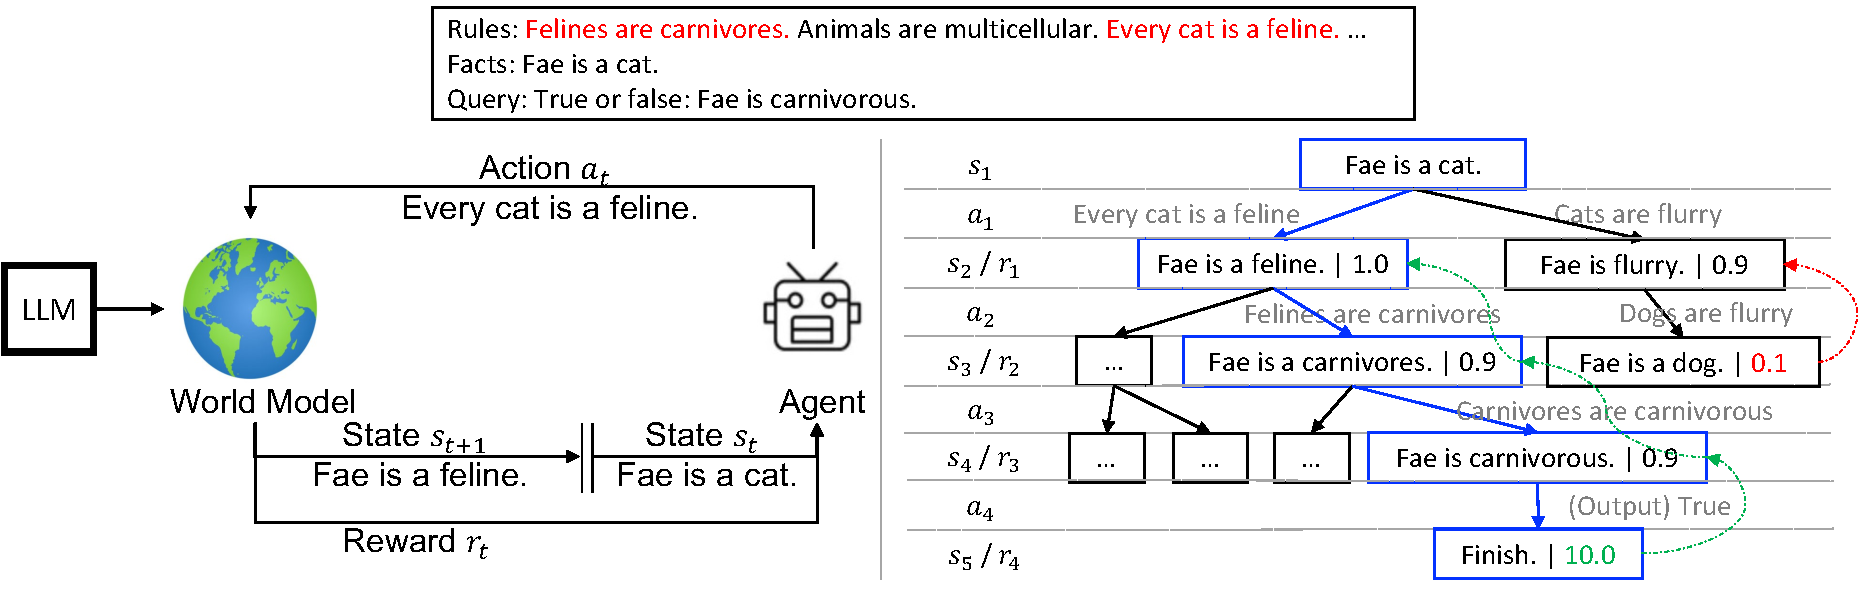
\includegraphics[width=\textwidth]{sections/fig_formulation.pdf}
%     \caption{Formulation of RAP in an example from PrOntoQA. The left is the formulation of LLM as World Model, and the right is a search tree in this example.}
%     \label{fig:formulation}
% \end{figure}

In general, a world model predicts the next \emph{state} of the reasoning after \roundinlinebox[green]{applying an \emph{action} to the current state}~\cite{ha2018world, matsuo2022deep}. \ours enables us to instantiate the general concepts of state and action in different ways depending on the specific reasoning problems at hand (Figure \ref{fig:tree_examples}). For example, in \blocksworld, it is natural to define a state as the configuration of blocks (described in natural language), and an action to be a behavior of moving a block (e.g., ``pickup the orange block''). In a math reasoning problem, we use the state to represent the values of intermediate variables, and set an action to be a subquestion that drives the reasoning to derive new values. In logical reasoning, a state is a fact we are focusing on, and an action is to choose a rule for the next deduction.


With the definition of state and action, the reasoning process can thus be described as a \highlight[green]{Markov decision process (MDP): given the current state $s_{t, t=0, 1, \dots, T}$, e.g., the initial state $s_0$, the LLM (as a reasoning agent) generates an action space by sampling from its generative distribution $a_t \sim p(a | s_t, c)$, where $c$ is a proper prompt (e.g., in-context demonstrations). Once an action is chosen, the world model then predicts the next state $s_{t+1}$ of the reasoning. Specifically, we repurpose the \emph{same} LLM to obtain a state transition distribution $p(s_{t+1} | s_t, a_t, c')$, where $c'$ is another prompt to guide the LLM to generate a state. For instance, in \blocksworld, the LLM (as the world model) generates text $s_{t+1}$ to describe the new configuration of blocks, given previous state $s_{t}$ and the action $a_t$}.

Continuing the process results in a reasoning trace, which consists of a sequence of interleaved states and actions $(s_0, a_0, s_1, \dots, a_{T-1}, s_T)$. This differs from the previous reasoning methods, such as Chain-of-Thought~\cite{wei2022chain}, where the intermediate reasoning steps consist of only a sequence of actions, e.g., (\texttt{$a_0=$ ``pickup red block'', $a_1=$ ``stack on yellow block'',} \dots) (see comparisons in Figure~\ref{fig:1}). Augmenting the reasoning with the (predicted) world states helps the LLM with a more grounded and coherent inference. Note that the full reasoning trace is simulated by the LLM itself (as a reasoning agent with an \emph{internal} world model) without interacting with the \emph{external} real environment. \highlight[green]{This resembles humans contemplating a possible plan in their minds. The capability of simulating future states, by introducing the world model, allows us to incorporate principled planning algorithms to efficiently explore the vast reasoning space} as described in Section~\ref{sec:mcts}.


% To introduce the world model for simulating reasoning traces, we begin by defining the concepts of \textit{states} and \textit{actions} within a reasoning task.
% % We illustrate this with an example taken from the PrOntoQA dataset \cite{saparov2022language}, as shown in Figure \ref{fig:formulation}.
% We illustrate this with an example derived from the \blocksworld benchmark \cite{valmeekam2022large}.
% In our approach, we represent the reasoning process as a Markov decision process (MDP) with a state space $\mathcal S$ and an action space $\mathcal A$, as depicted in Figure \gy{ref figure}. %\ref{fig:formulation} (left).
% Each state $s \in \mathcal S$ corresponds to an intermediate status in the reasoning, specifically a language description of the current configurations of blocks in the \blocksworld context. %``\texttt{Fae is a cat}''.
% % At time $t$, an agent proposes an action $a_t \in \mathcal A$, which represents a rule to be employed in the subsequent reasoning step, such as ``\texttt{Every cat is a feline}'', based on the current state $s_t$ and its policy $p_\phi(a \mid s_t)$.
% At time $t$, an agent proposes an action $a_t \in \mathcal A$, which represents the subsequent reasoning step, such as a movement of a single block, based on the current state $s_t$ and its policy $p(a \mid s_t)$.
% The world model then conducts a one-hop reasoning step using $s_t$ and $a_t$, transitioning the state into the subsequent state $s_{t+1}$, which in this case denotes the new configuration of blocks after performing the movement $a_t$ on the current configuration $s_t$.
% The specific definition of states and actions can vary depending on the nature of the reasoning task.
% For example, in GSM8k \cite{cobbe2021training}, a dataset of numerical reasoning, the action is defined as proposing an incremental sub-question, while the state comprises the history of previous sub-questions and their corresponding answers.
% In terms of state transition, the world model attempts to answer the sub-question based on the problem context and the current state, subsequently incorporating the answer into the history to form the next state.

% In order to enable the world model to predict state transitions, which are subsequently utilized by agents for planning, we leverage the LLM as the state transition probability function $p_\theta$.
% In the \blocksworld example, we prompt the LLM the domain rule, the state $s_t$, the action $a_t$, and few-shot examples, to predict the next state $s_{t+1}$.




% In the PrOntoQA example, we prompt the LLM the state $s_t$ and action $a_t$ with few-shot examples to get the next state $s_{t+1}$.
% We also prompt it ``\texttt{Is this reasoning step correct?}'', and use the probability of ``\texttt{Yes}'' as the reward, evaluating the correctness of this reasoning step.

%However, the LLM often makes mistakes in retrieving accurate information or performing correct mathematical calculations.
%To ensure the reliability of our world model, we sample the LLM multiple times and select the next state with the highest confidence (The frequency of an answer). \gy{OK to directly say confidence?}
%We also use this confidence value as a reward, discouraging excessively difficulty or skipping sub-questions.

% In plan generation tasks, the world model is used to simulate actions by predicting the state transitions and the rewards without requiring direct access to the environment.
% In numerical and logical reasoning tasks, the LLM is utilized to answer sub-questions and perform atomic logical reasoning steps, allowing us to learn the outcome of reasoning steps and providing evaluations how good they are.
% Through the integration of the world model, a reasoning task is transformed into a strategic planning problem over the MDP, guided by the rewards.

% To address this, we employ a LLM as the world model, leveraging it to simulate the state transition function and the reward function.
% In abstract reasoning tasks \gy{unsure how to describe this type}, the definition of states and actions are more flexible.
% A partial solution $s \in \mathcal S$ can correspond to an intermediate conclusion or the previous answers of decomposed sub-questions. A reasoning step $a \in \mathcal A$ can refer to a given fact or a new sub-question that leads to the next state.
% In these cases, we also utilize a LLM as the world model to simulate the state transition, enabling us to derive the next intermediate conclusion or answer the sub-question. We also evaluate the quality of each reasoning step using the LLM as the reward function.
% We illustrate the detailed MDP formulations of Blocksworld, ProntoQA, and GSM8k in \gy{table/figure}. \gy{we want to include action proposing in world model, need modify}

% We assume the MDP has finite horizon, which means any transition sequence of nonzero probability (i.e. $ \prod_{i \geq 0} \mathcal{P}\left(x_i, a_{i, i+1}, x_{i+1}\right)>0$) must have finite length.
% Since their concrete interpretations of the MDP depend on specific problems, we leave them to later sections \hsb{ref}. Here we take a case from blockworld as a running example: \hsb{expand}

% In our method, the transition probability function and the reward function are parameterized by the world model, noted as $\mathcal{P_\phi}$ and $\mathcal{R_\phi}$. \hsb{example}

% A planning problem is formulated as below:


%\vspace{-5pt}
\subsection{Reward Design} \label{sec:reward}
%\vspace{-5pt}

During reasoning, we want to assess the feasibility and desirability of each reasoning step, and guide the reasoning based on the assessment (Section~\ref{sec:mcts}).
The assessment of each reasoning step (i.e., applying an action $a_t$ to the state $s_{t}$) is performed by a \emph{reward} function $r_t = r(s_t, a_t) \in \mathbb R$. Similar to the state and action, the reward function can be specified in different ways to accommodate any knowledge or preferences about the reasoning problem of interest. Here we introduce several common rewards applicable to different tasks and shown to be effective in our experiments.

\noindent \textbf{Likelihood of the action.}
When an action is generated by the LLM conditioning on the in-context demonstration and the current state, the probability of the specific action reflects the LLM's preference. We thus can incorporate the log probability of the action as a reward. This reward reflects the ``instinct'' of LLMs as an agent, and can be also used as a prior for which action to explore.

\noindent \textbf{Confidence of the state.}
State prediction is nontrivial in some problems, e.g., in math reasoning (Figure~\ref{fig:tree_examples}, middle), given an action (i.e., a subquestion), the world model predicts the next state by answering the subquestion. We incorporate the confidence of the state (i.e., answers in this case) as a reward. Specifically, we draw multiple sample answers from the world model, and use the proportion of the most frequent answer as the confidence. Higher confidence indicates that the state prediction is more consistent with the world knowledge of LLMs \cite{hao2023bertnet}, which typically leads to a more reliable reasoning step.

% In certain tasks, individual reasoning step can still be challenging.
% For example, in the GSM8k dataset \cite{cobbe2021training}, a reasoning step involves proposing (action) and answering a sub-question (state transition) based on previous information.
% We then use the confidence of answers as a reward. Specifically, we sample multiple responses from the world model and group them by the answer. The maximal frequency of an answer is defined as confidence, and high confidence indicates reliable reasoning steps.

% \textbf{Correctness estimation by LLM. \gy{Since we use this way to calculate correctness in PrOntoQA and helpfulness in GSM8k, shall we replace with `Self-evaluation by LLM'} \hzt{sounds good. and please update the paragraph}}
\noindent \textbf{Self-evaluation by the LLM.}
It's sometimes easier to recognize the errors in reasoning than avoid generating them in advance. Thus, it's beneficial to allow the LLM to criticize itself with the question ``\texttt{Is this reasoning step correct?}'', and use the next-word probability of the token ``\texttt{Yes}'' as a reward. The reward evaluates LLM's own estimation of the correctness of reasoning. Note that the specific problems for self-evaluation can be different depending on the tasks.

% Likewise, we can prompt the LLM with the question ``\texttt{Is this reasoning step correct?}'' and utilize the probability of the token \texttt{Yes} as a reward, reflecting the LLM's evaluation of the reasoning step's reliability,

\noindent \textbf{Task-specific heuristics.}
RAP also allows us to flexibly plug in other task-specific heuristics into the reward function. For example, in plan generation for \blocksworld, we compare the predicted current state of blocks with the goal to calculate a reward (Section~\ref{sec:plan}). The reward encourages the plan of movements to actively pace towards the target.

% In plan generation tasks, we can also borrow the rewards from the corresponding environment. For example, in \blocksworld benchmark \cite{valmeekam2022large}, we can assign reward by the number of sub-goals that are fulfilled when performing the movement in action $a_t$.

% As a by-product, the new state is predicted as the ensemble of multiple samples, which may better align with the LLM's belief about the world \cite{jung2022maieutic, hao2022bertnet}.



% Besides the world model, we define a reward function $r_t = r(s_t, a_t) \in \mathbb R$ for each task to assess the quality of this reasoning step.
% The reward function can incorporate various evaluation approaches, some of which are outlined below.

% \vspace{-5pt}
\subsection{Planning with Monte Carlo Tree Search} \label{sec:mcts}
% \vspace{-5pt}


\begin{figure*}[t]
    \centering
    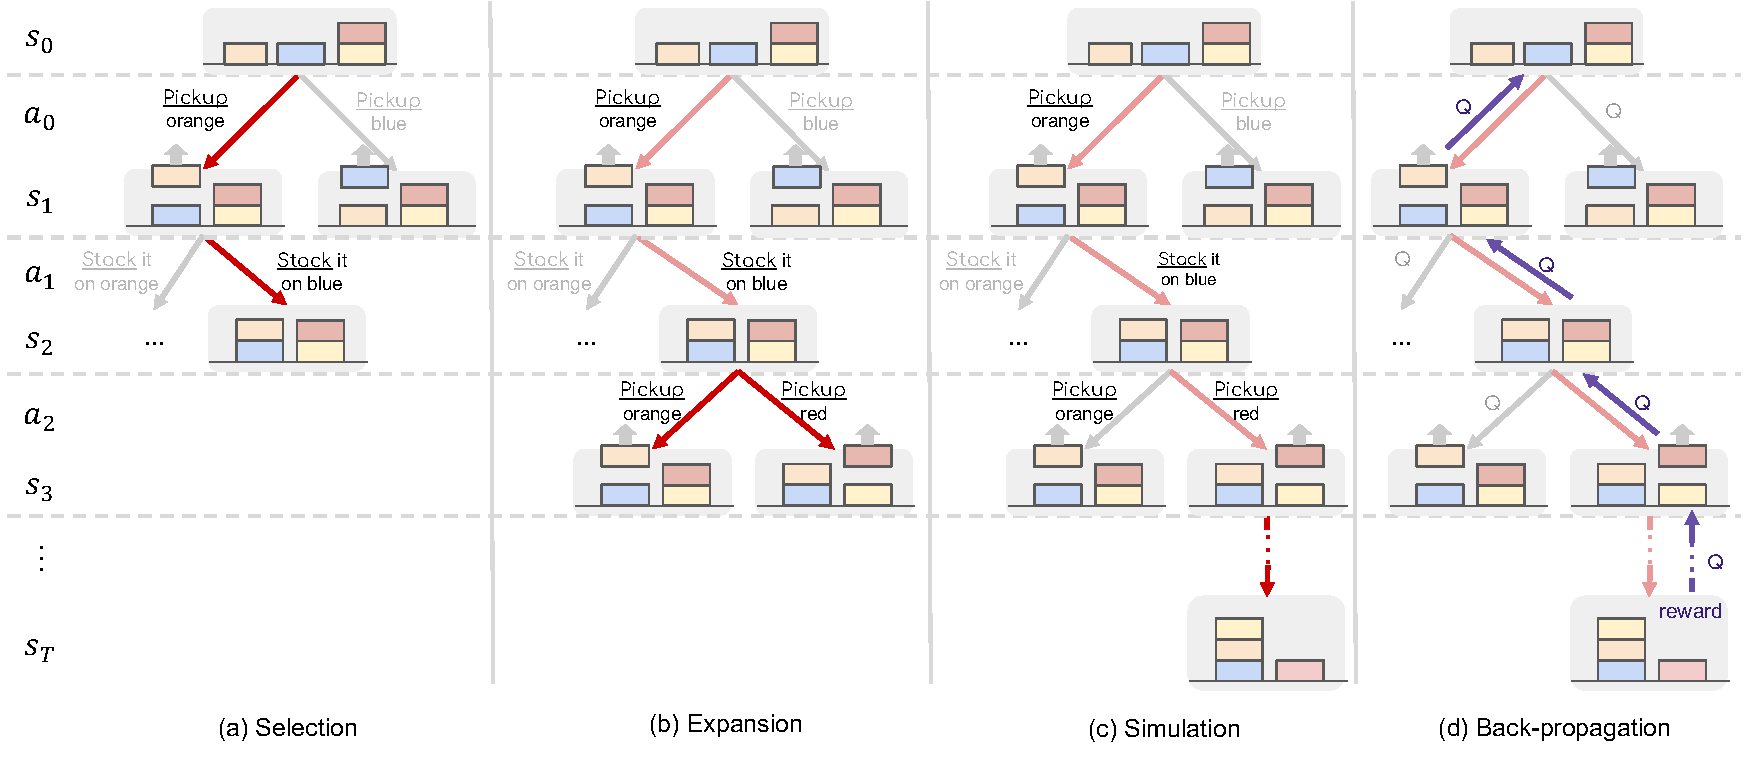
\includegraphics[width=\textwidth]{sections/mcts_phases.pdf}
    \vspace{-25pt}
    \caption{An illustration of the four phases in an iteration in MCTS planning (Section~\ref{sec:mcts}).}
    \label{fig:mcts_phases}
    \vspace{-12pt}
\end{figure*}


Once equipped with the world model (Section~\ref{sec:formulation}) and rewards (Section~\ref{sec:reward}), LLMs can reason with any planning algorithms. We adopt Monte Carlo Tree Search (MCTS)~\cite{kocsis2006bandit, coulom2007efficient}, a powerful planning algorithm that strategically explores the space of reasoning trees and strikes a proper balance between exploration and exploitation to find high-reward reasoning traces efficiently.

Specifically, MCTS builds a reasoning tree iteratively, where each node represents a state, and each edge represents an action and the transition from the current state to the next state after applying the action (Figure~\ref{fig:1}).
To guide the LLM agent to expand and explore the most promising nodes of the tree, the algorithm maintains a state-action value function $Q : \mathcal S \times \mathcal A \mapsto \mathbb R$, where $Q(s, a)$ estimates the \emph{expected future reward} of taking action $a$ in state $s$. Figure \ref{fig:mcts_phases} illustrates four operations in each iteration to expand the tree and update $Q$ values. The process continues until a specified computational budget (e.g., the number of iterations) is reached, and the resulting traces are acquired from the tree. More details and the pseudo-code of the planning algorithm are given in Appendix~\ref{sec:mcts_app} and Algorithm \ref{alg:mcts}.


% That is, we assess the potential of a node (a reasoning step) by looking ahead and anticipating the reward in future trajectories starting from this node. This fundamentally differs from the current reasoning methods that generate a reasoning trace autoregressively without considering the future.


% More specifically, as illustrated in Figure \ref{fig:mcts_phases}, the MCTS planning performs four operations in each iteration to expand the tree and update $Q$ values, i.e., \textit{selection}, \textit{expansion}, \textit{simulation}, and \textit{back-propagation}. The process continues until a specified computational budget (e.g., the number of iterations) is reached, and the resulting reasoning traces are acquired from the tree, as we articulated later. The psuedo-code of our MCTS planning is given in Algorithm \ref{alg:mcts} in the Appendix.
% The iterations continue until a target state is reached, resulting in a complete reasoning trace for the target problem.

% We employ Monte Carlo Tree Search (MCTS), a decision-making algorithm that explores the MDPs using a decision tree, by which we can balance exploration and exploitation when planning the reasoning trace. In the decision tree representation, each node represents a state, while each edge represents an action and the corresponding state transition, as illustrated in Figure \ref{fig:formulation} (right).

% The algorithm maintains an optimal state-action value function $Q : \mathcal S \times \mathcal A \mapsto \mathbb R$, where $Q(s, a)$ estimates the maximum expected reward starting from state $s$ with action $a$.
% MCTS operates iteratively by sampling a complete trajectory (i.e., a reasoning trace) from the root of the tree (initial state $s_0$) towards a terminating node, where the agent finishes the reasoning.
% This iterative process expands the decision tree incrementally with each iteration.
% Additionally, the $Q$ values of the state-action pairs along the trajectory are updated in each iteration.
% Every iteration is composed four phases, \textit{selection}, \textit{expansion}, \textit{simulation}, and \textit{back-propagation}, demonstrated in Algorithm \ref{alg:mcts} with details below.

% In reasoning tasks, the state space and action space of half-way solutions can be very large and even infinite due to the flexibility to propose reasoning steps in natural language, which means that the state space cannot be fully searched.
% In order to do planning on the MDP within a computational budget, we introduce the Monte Carlo Tree Search algorithm \cite{browne2012survey} to strategically and efficiently search for a good plan.
% The algorithm builds a rooted tree of the search history, where each node represents a state, while each edge represents an action.
% It also maintains an optimal state-action value function $Q: \mathcal S \times \mathcal A \mapsto \mathbb R$, which will be used in roll-out policy.
% The algorithm will do several iterations, called roll-outs, each of which consists of the following four phases.
% We present the roll-out procedure in Algorithm \ref{alg:mcts} with psuedo-code.

\noindent \textbf{Selection.}
The first phase selects a portion of the existing tree that is most promising for further expansion in the next phase. Starting from the root node (i.e., initial state $s_0$), at each level of the tree, the algorithm selects a child node as the next node. The phase finishes when a leaf node of the current tree is reached. Figure~\ref{fig:mcts_phases}(a) highlights the selected path in red. To balance between exploration (of less-visited nodes) and exploitation (of high-value nodes), we use the well-known \emph{Upper Confidence bounds applied to Trees (UCT)} \cite{kocsis2006bandit} to select each child node. Specifically, at node $s$, we select the action in the tree by considering both the $Q$ value (for exploitation) and uncertainty (for exploration):

\vspace{-8pt}
{
\small
\begin{align}
    a^\ast = \arg\max_{a \in A(s)} \left[ Q(s, a) + w \sqrt{\frac{\ln N(s)}{N(c(s, a))}} \right],
\end{align}
}
\noindent where $N(s)$ is the number of times node $s$ has been visited in previous iterations, and $c(s, a)$ is the child node of applying $a$ in state $s$. The less a child node was visited before (i.e., the more uncertain about this child node), the higher the second term in the equation. The weight $w$ controls the balance between exploration and exploitation.
% \hzt{Anything to say about how we chose $w$?}

% Each iteration starts the initial state.
% In each step, the algorithm will select a child node based on a \textit{tree policy}, until reaching an unvisited node.
% To balance between exploration and exploitation, we use the maximum Upper Confidence Trees (UCT) policy, which select the child node based on maximizing upper confidence.
% The upper confidence is determined by the summation of the $Q$ value, which encourages exploitation, and an uncertainty term, which encourages exploration.
% \begin{align}
%     a^\ast = \arg\max_{a \in A(s)} \left[ Q(s, a) + w \sqrt{\frac{\ln N(s)}{N(c(s, a))}} \right],
% \end{align}
% where $N(s)$ is the number of times node $s$ has been visited, and $c(s, a)$ is the children of following $a$ at node $s$.
% The hyper-parameter $w$ serves as a balancing factor between exploration and exploitation.

\noindent \textbf{Expansion.}
This phase expands the tree by adding new child nodes to the leaf node selected above. Given the state of the leaf node, we use the LLM (as agent) to sample $d$ possible actions (e.g., subquestions in math reasoning), and then use the LLM (as world model) to predict the respective next state, resulting in $d$ child nodes. Note that if the leaf node selected above is a terminal node (the end of a reasoning chain) already, we will skip expansion and jump to back-propagation.
% Note that if the leaf node selected above is a terminal (target) state already, we will skip expansion/simulation and jump to back-propagation.

% When reaching a node that have never been visited, we add to the tree the children of the node.
% Since the space of language representations can be very large, we sample $d$ possible actions using the LLM as a substitute action space $A(s)$, and add the $d$ corresponding children to the tree.

% Since the space of action, which is a language representation of the next reasoning step, can be very large, we sample $d$ possible actions using the world model LLM as the children, where $d$ is a pre-defined hyper-parameter.
% To simplify the problem, we sample a next state using the transition probability function, and reuse the sample in the future.
% The difficulty of predicting state transitions vary among tasks.
% For easier transitions, we to generate the next state with greedy decoding, while for harder transitions, we utilize self-consistency, which means we use the next state with highest confidence across several generations.
% We will also have a quick evaluation of each action, namely a prior $r'$, which can be but not necessarily be the reward defined in the world model.
% We use $r'$ to temporarily serve as $Q(s, a)$ before a roll-out actually follows $a$ at the node representing the state $s$.

\noindent \textbf{Simulation.}
To estimate the expected future rewards ($Q$ values), this phase simulates the future situations of the current node using the world model.
% Specifically,
%from the above $d$ new nodes, we pick the node of largest local reward (Section~\ref{sec:reward}) and perform simulation starting from it. In particular, similar to above,
Starting from the current node as above, at each node $s$, we create an action following a \emph{roll-out policy} and use the world model to predict the next state. The roll-out process continues until a terminal state is reached. There could be many ways to define the roll-out policy (e.g., by adding different randomness). In our experiments, for simplicity and reduced noises, we follow a similar process as in the expansion above, i.e., generating $d$ candidate actions and picking one of the largest local reward $a'= \max_{a'} r(s, a)$. In practice, for efficiency, we discard the computationally costly components in $r$ (e.g., the reward from the confidence of state requires sampling the answer multiple times), and use the resulting lightweight reward function for selecting actions during simulation.

% In traditional MCTS algorithms, after expanding the children of one node, it will follow a random simulation till a terminating state, i.e., a leaf node.
% To encourage efficient exploration, we instead follow the children with the highest prior $r'$, and repeat this procedure after expanding the new visited node till the end.


% After expansion, we perform a complete simulation starting from the current node until the reasoning trace is finished following a \textit{roll-out policy}. To guide our exploration towards better reasoning traces, we use a fast reward function $r'(s, a)$, discarding time-consuming parts of the standard reward function $r(s, a)$, to get an estimation of the quality of action $a$. Our roll-out policy selects the action with maximum estimated reward $a_t = \max_{a_t} r'(s, a_t)$.

\noindent \textbf{Back-propagation.}
Once we reach a terminal state in the above phases, we obtain a reasoning path from the root node to the terminal node. We now back-propagate the rewards on the path to update the $Q$ value of each state-action pair along the path. Specifically, we update $Q(s, a)$ by aggregating the rewards in all future steps of node $s$.
% We may adopt the aggregation method depending on the nature of tasks and reward design, as discussed in Section~\ref{sec:experiments}.
% After an iteration reaches a terminal state in the above phases.
% We back propagated the rewards on the path, updating the $Q$ function with each state-action pair in the trajectory with rewards in all future steps.
% Since the $Q$ function depends on the reward design, we will introduce in detail in Section \ref{sec:experiments}.

Once a predetermined number of MCTS iterations is reached, we terminate the algorithm and select the final reasoning trace from the constructed tree for evaluation. There are various ways for the selection.
% Following a predetermined number of iterations, there are several strategies for selecting the final reasoning path.
One is to start from the root node and iteratively choose the action with the highest $Q$ value until reaching a terminal.
Also, one can directly select the path from the iterations that yielded the highest reward, or opt to choose the leaf node (and the respective root-to-leaf path) that has been visited the most.
In practice, we observed that the second strategy often yields the best results.

% When solving a reasoning problem in the task, we deploy an agent to search over the corresponding MDP.
% In order to keep a track of the searching history, we build a reasoning tree representing the progress of searching.
% Each node on the tree represents a state $S \in \mathcal S$ in the MDP, where the root represents the initial state $S_0$.
% Every time the agent reaches a new node $S_t$ on the tree,

%\vspace{-5pt}
\subsection{RAP-Aggregation} \label{sec:aggr}
%\vspace{-5pt}

% : Aggregating Multiple Reasoning Outputs

For problems, such as math reasoning (Section~\ref{sec:math}) where only the final answer is required, \ours could produce multiple traces and answers from different MCTS iterations, which will be aggregated to produce the final answer. We refer to such a mechanism as \ours-Aggregation. Note that problems like plan generation or logical inference require a complete reasoning trace as output; thus, \ours-Aggregation will not be applied.

% More importantly, there is a concern that some incorrect reasoning steps may appear in the early stage of multiple iterations, thus polluting the aggregation. As a result, we further devise a new weighting strategy for aggregating candidate answers. Specifically, for each candidate answer, we accumulate the reward of each reasoning step in the answer's reasoning traces. We choose the answer with the highest accumulative reward as the final aggregated answer.


% Some of the reasoning problems, such as plan generation (Section~\ref{sec:plan}) and logical inference (Section~\ref{sec:logical}), require a complete reasoning trace as output. In other problems, such as math reasoning (Section~\ref{sec:math}), only the final answer is required. In such cases, we could collect multiple reasoning traces during RAP and aggregate the respective answers to produce the final answer, similar to the self-consistency method \cite{wang2022self} in Chain-of-Thought.
% Specifically, we collect reasoning traces and answers from different MCTS iterations. To address the concern that some incorrect early reasoning steps may appear in multiple iterations and thus pollute the aggregation, we devise a new  weighting strategy for aggregating candidate answers. Specifically, for each candidate answer, we accumulate the reward of each reasoning step in the answer's reasoning traces. We choose the answer with the highest accumulative reward as the final aggregated answer.

% However, in certain tasks such as many numerical reasoning tasks, only the final answer needs to be provided.
% When tackling numerical reasoning problems, humans often consider multiple reasoning paths to verify the answer further.
% Inspired by this, we introduce \textbf{RAP-aggregation}, where we aggregate the answer across iterations to enhance the output of MCTS.
% To address the concern that an early incorrect reasoning step may contribute multiple times to the final result when it appears in multiple iterations, we perform the aggregation in a basis of edges.
% Specifically, for a given potential answer, we accumulate the weights of all edges involved in at least one iteration leading to that particular answer.
% The weight of an edge is the reward assigned to its represented action.
% Ultimately, the answer with the highest total weight is selected as the aggregated output.
% To avoid an early incorrect reasoning step contributing multiple times to the result when multiple iterations include that step, we conduct the vote by edges.
% More specifically, for one possible answer, all edges involving in at least one iteration with that final answer will be added to the weight for the answer, and the weight is the reward of the action represented by the edge.


% Formally, we choose the answer $o$ following
% \begin{align}
%     o^\ast = \arg\max_{o} \sum_{e = (s, a): \exists T: T\text{~outputs~}o \wedge e \in T} r(s, a),
% \end{align}
% where $e$ is an edge on the tree representing following action $a$ when visiting the node representing $s$, and $T$ is the trace in one roll-out.


%\vspace{-5pt}
\section{Experiments} \label{sec:experiments}
%\vspace{-5pt}


In this section, we demonstrate the flexibility and effectiveness of our RAP framework by applying it to a wide range of problems, including plan generation in an embodied environment (\ref{sec:plan}), mathematical reasoning for solving math word problems (\ref{sec:math}), and logical reasoning for verifying hypotheses (\ref{sec:logical}). The subsequent sections demonstrate how the world model formulation in RAP enables a versatile design of the state and action, catering to various reasoning contexts.

We primarily compare RAP with chain-of-thought (CoT)~\cite{wei2022chain}, and its variants like least-to-most prompting~\cite{zhou2022least} as baselines. We also consider ensembling multiple reasoning paths if applicable (also known as self-consistency~\cite{wang2022self}). Moreover, we compare \ours with GPT-4~\cite{openai2023gpt4} when computation resources allow. By default, we use the LLaMA-33B model \cite{touvron2023llama} as the base LLM for both our methods and baselines, with a sampling temperature of 0.8. All prompts are listed in Appendix~\ref{sec:prompt}.

% benefits from the adaptable design of the state and action components within the world model formulation, enabling its application to diverse reasoning tasks.
% In this section, we illustrate the adaption of our RAP framework to plan generation, numerical reasoning, and logical reasoning tasks, and provide a comparative analysis of the results against CoT \cite{zhou2022least} and least-to-most \cite{wang2022self} prompting.
% We implement our framework and baselines with LLaMA-33B model \cite{touvron2023llama}, and use a temperature of 0.8 for sampling.

%\vspace{-5pt}
\subsection{Plan Generation} \label{sec:plan}
%\vspace{-5pt}


\begin{figure*}
    \centering
    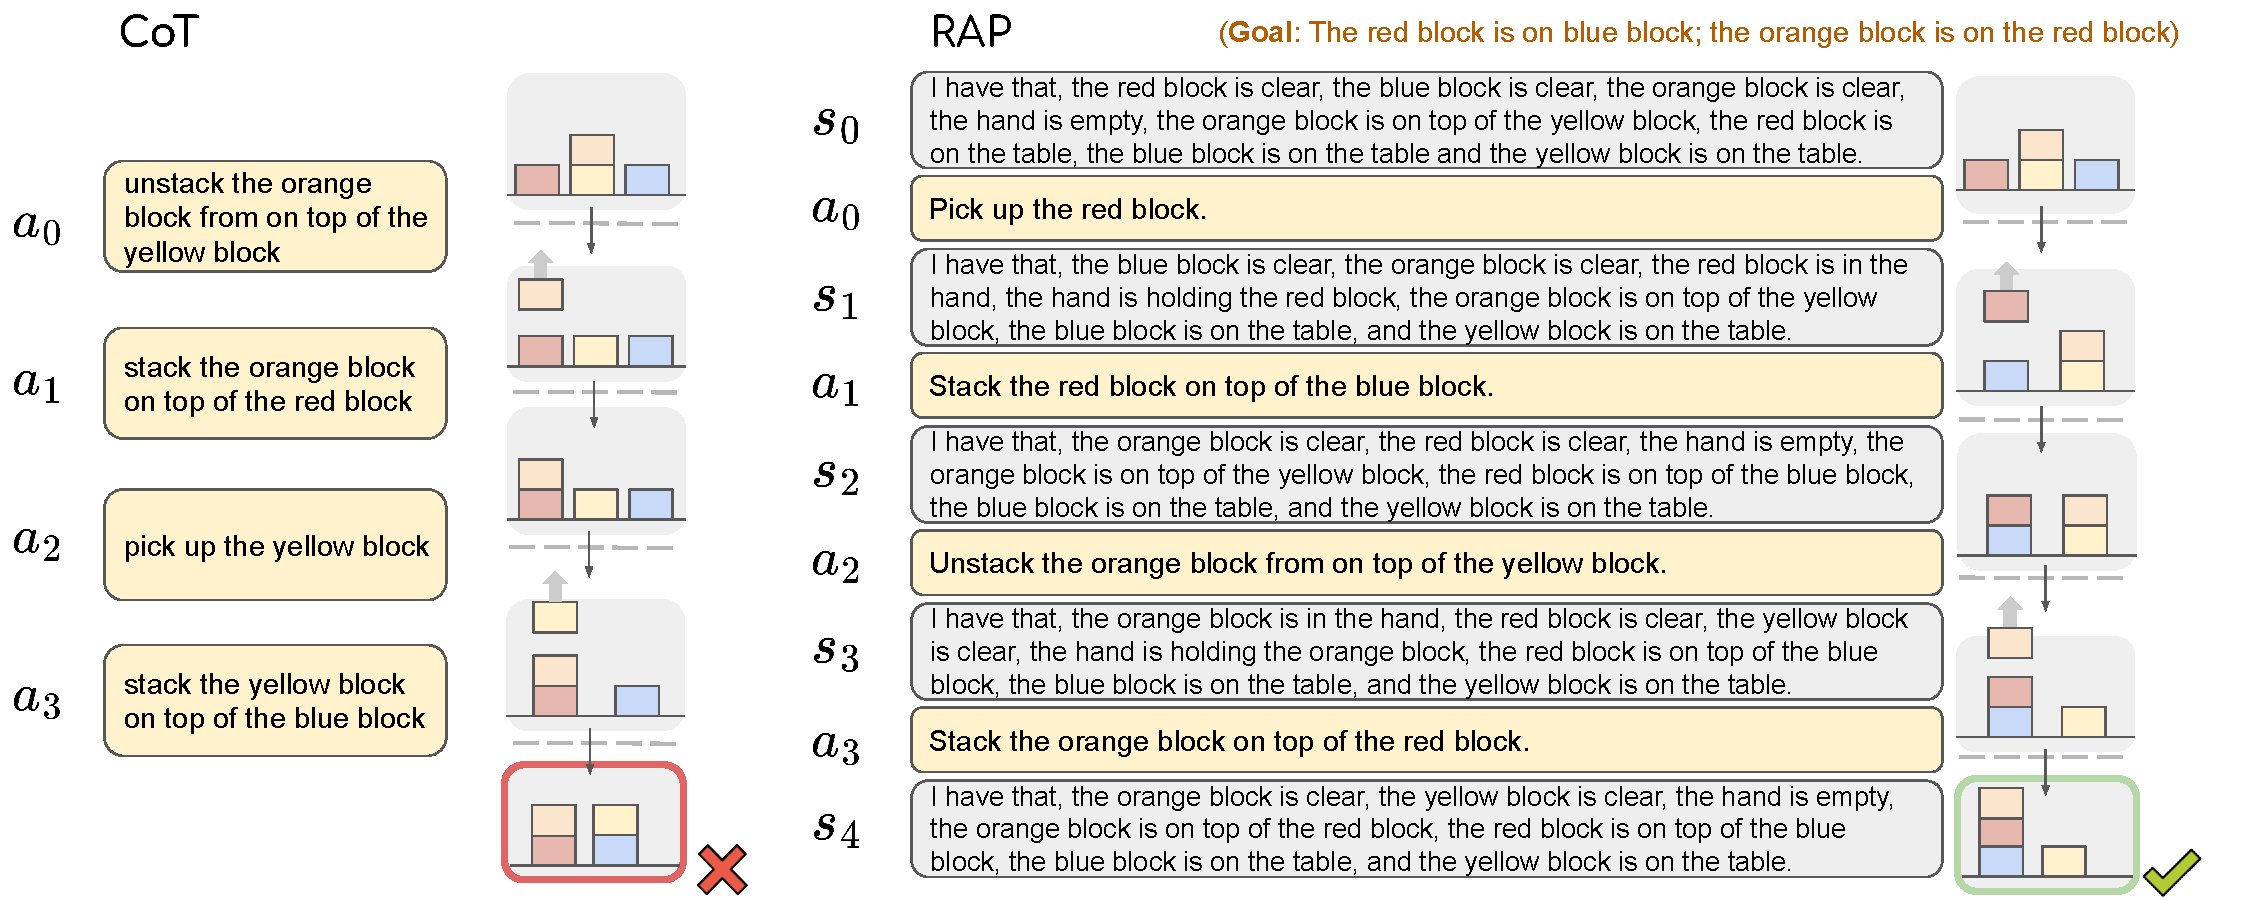
\includegraphics[width=0.9\textwidth]{sections/Figure-4_final.pdf}
    \vspace{-8pt}
    \caption{Comparing reasoning traces in \blocksworld from CoT (left) and \ours (right).}
    \label{fig:bw_example}
    \label{fig:my_label}
    \vspace{-12pt}
\end{figure*}



The plan generation task aims to produce a sequence of actions to achieve a given goal, possibly with additional constraints. The ability to generate plans is important for intelligent embodied agents, e.g. household robots~\cite{puig2018virtualhome}. % such as VirtualHome \cite{puig2018virtualhome} and \blocksworld \cite{valmeekam2022large}. 
% This task has also been widely used to evaluate the reasoning ability of LLMs given their challenging requirements of long-horizon reasoning, e.g., \blocksworld is a classic problem, where an agent is asked to rearrange the blocks into stacks in a particular order. 

% In these tasks, a plan is expected to be executable, meaning that each step in the plan must be valid when considering the conditions. \hsb{I feel that we don't need to emphasize the validity of actions, as that's not what we want to solve with RAP}
% In the \blocksworld domain where steps are actions that move blocks, an executable plan implies that each step is valid when considering the state of the blocks before the step (for instance, picking up a block is not allowed when there is already a block in the hand). 
% While not all plan generation tasks can be broken up into discrete steps, those that can provide a natural approach for adapting the RAP framework.
% what do we want to deliver with this sentence?
% As each step in a plan induces change in the current conditions, we formulate the set of conditions as the state of the world and individual steps as being state transitions.
%\hzt{Some of the discussions are too abstract. Perhaps use Blockworld as example.}

% \hzt{Need a figure to illustrate how the problem is mapped to our formulation. Refer to the figures in "Tree of Thoughts" in each experiment section.}

\noindent \textbf{Task setup.}
% \paragraph{Task setup.} 
To explore the viability of the RAP framework for plan generation tasks, we adapt and evaluate RAP on the \blocksworld benchmark~\cite{valmeekam2022large}, where an agent is asked to rearrange the blocks into stacks in a particular order. 
% This domain consists of a set of colored blocks that are either on top of a table or on top of another block. 
% With the goal being to reach an orientation of the blocks that satisfy some given conditions, the task is to rearrange the blocks with a series of valid actions. 
We define a \textbf{state} as the current orientation of the blocks and an \textbf{action} as an instruction that moves blocks. Specifically, an action is composed of one of the 4 verbs (i.e., \textsc{Stack}, \textsc{Unstack}, \textsc{Put}, and \textsc{Pickup}) and manipulated objects. For the action space, we generate the currently valid actions given the domain restrictions on actions and the current orientation of the blocks. To transit between states, we take the current action and query the LLM to predict the state changes to the relevant blocks. We then update the current state by adding the new block conditions and removing the conditions that are no longer true. Once a state has met all conditions in the goal or the depth limit of the tree is reached, we terminate the associated node.

To assess the quality of actions within this domain, we use two separate \textbf{rewards}. 
First, we prompt the LLM with some example test cases along with their solutions, and then calculate the log probability of the action given the current state (\textit{``Likelihood of action''} reward in Section~\ref{sec:reward}), denoted as $r_{1}$. This reward reflects the intuition of the LLM as the reasoning agent. It's typically indicative when there are few steps left to the goal, while not as reliable for a distant goal. Additionally, we compare the new state after performing an action with the goal and provide a reward, $r_{2}$, scaling with the number of conditions met (\textit{``Task-specific heuristics''} reward). Specifically, when all the conditions are met, we assign a super large reward to make sure this plan will be selected as the solution. %While there may be multiple plans that correctly reach the given goal, a given state usually has a clear action that is most optimal. Therefore, we do not apply 

%Aggregation \hsb{refer} doesn't apply to this task, because unlike ..., here all the reasoning steps will be included in the plan. 
%\hsb{can we specify the scope of aggregation in section 3? i.e. only available for result-oriented problems}
%on the search tree and instead find the reasoning trace with maximum reward when returning the final plan.



\begin{table}[t!]
    \small
    \centering
    % \vspace{pt}
    \begin{tabular}{r c c c}
        \toprule
        \textbf{Method} & \textbf{2-step} & \textbf{4-step} & \textbf{6-step}\\
        \midrule
        CoT & 0.17 & 0.02 & 0.00\\
        %\multicolumn{1}{r|}{ - pass@10} & 0.23 & 0.07 & 0.00 \\ 
        CoT - pass@10 & 0.23 & 0.07 & 0.00 \\ 
        %\multicolumn{1}{r|}{ - w/ GPT-4} 
        CoT (GPT-4) & 0.50  & 0.63 & 0.40\\
        
        \midrule
        RAP$^{(10)}$ & 1.00 & 0.86 & 0.26 \\
        RAP$^{(20)}$ & \textbf{1.00} & \textbf{0.88} & \textbf{0.42} \\
        \bottomrule
    \end{tabular}
    % \vspace{4pt}
    \vspace{-5pt}
    \caption{Results on \blocksworld. RAP$^{(10)}$ and RAP$^{(20)}$ refer to our method where the iteration number is set to 10 and 20, respectively. ``pass@10'' means 10 plans are sampled for each test case, and the test case is regarded as solved if at least one plan is correct. All other settings including RAP, only evaluate a single plan.}
    \label{tab:bw}
    \vspace{-12pt}
\end{table}


\noindent \textbf{Results.}
% \paragraph{Results.}
%We evaluate our framework on Blockworld, with the task being to generate a valid plan that reaches a goal given an initial state. 
We use test cases from the \blocksworld dataset \cite{valmeekam2023planning} and group them by minimum number of actions required, resulting in 30 cases solvable within 2 steps, 57 cases within 4 steps, and 114 cases within 6 steps.
% We also conduct experiments on the more challenging full Blocksworld with a stronger LLM in section \ref{sec:bw_appendix_full}.
There are at most 5 blocks in each test case. As the baseline method, we prompt the LLM with 4 test cases with corresponding solutions, and ask it to generate a plan for a new question. This setting is the same as one described in \citet{valmeekam2022large}, and we denote it as Chain-of-Thought (CoT) as the solution is generated step by step. For RAP, the same prompt is shown to help LLMs calculate $r_1$. 

As shown in Table~\ref{tab:bw}, CoT with LLaMA-33B can only generate successful plans for a few 2-step cases, and completely fails on harder problems. RAP substantially improves over CoT by nearly solving all problems within 4 steps, and a part of 6-step problems, achieving an average success rate of $64\%$. It's worth noting that the searching space of 6-step problems can be as large as $5^6$, while our algorithm can find a successful plan 42\% of the time within 20 iterations. Even more, our framework allows LLaMA-33B to outperform GPT-4 by $33\%$ relative gain, which is known to have much stronger reasoning ability~\cite{bubeck2023sparks}. %\footnote{For some unknown reasons, GPT-4 tends to generate long plans.}.


\noindent \textbf{Case study.}
We compare the reasoning paths from CoT and \ours in Figure~\ref{fig:bw_example}. We summarize the reasons accounting for the improvement: (1) By maintaining the world state during reasoning, RAP can recognize valid actions for the current state, avoiding generating illegal plans. (2) RAP is capable of backtracking and trying out other solutions when the first intuition from the LLM doesn't work. Specifically, CoT attempts to achieve the second goal, i.e. ``orange on red'', and achieve that with the first two steps. However, accomplishing the second goal first would prevent the first goal from being satisfied. On the contrary, even though RAP makes the same mistakes in the first iterations, our framework drives the agent to explore other possible paths (as described in Section~\ref{sec:mcts}) and finally generate a successful plan. (3) When calculating $r_t$, we can only feed the current state to the LLM and hide the history. E.g., in the case of Figure~\ref{fig:bw_example}, to calculate the reward for $a_2$, the LLM is provided with a ``new'' test case, in which $s_2$ is the initial state. This significantly lowers the difficulties of the last few steps, and saves more iterations for harder decisions of the first few steps.

%We take these instances from a dataset of problems that consist of a maximum of 5 blocks in each 
% shibo: I just checked the dataset and there are actually cases with 5 blocks.
%problem. With these instances, we further sort the problems based on the optimal number of steps needed to reach the goal. We use FILLER-shot examples for both our framework and the baselines, and do FILLER roll-outs in MCTS. \jjh{FILL will data + analysis}

% \vspace{-5pt}
\subsection{Math Reasoning} \label{sec:math}
% \vspace{-5pt}


\noindent \textbf{Task setup.}
% \paragraph{Task setup.} 
Math reasoning tasks, such as GSM8k \cite{cobbe2021training}, often include a description and a final question.
To arrive at the answer to the final question, it is necessary to undertake multi-step mathematical calculations 
%on the numbers provided in the description 
based on the problem's context.
It is thus natural to decompose the final question into a sequence of smaller sub-questions (Figure~\ref{fig:tree_examples}, right).
% \textcolor{blue}{
We define a \textbf{state} as the values of intermediate variables,
and an \textbf{action} as to propose an incremental sub-question about a unknown intermediate variable.
% To adapt RAP, we define a state as the already answered sub-questions \hzt{we shall say the state is the values of intermediate variables, and in implementation, instead of defining a new format, we simply stack all subquestions and their answers together to represent the state}, while an action is to propose a new sub-question.
The world model then responds to the sub-question using the intermediate variables and the problem description, adding the new intermediate variable value into the next state.
% For state transitions, the world model leverages the answers from previous sub-questions in the current state to respond to the new sub-question and incorporates it, along with its answer, into the next state \hzt{This sentence is long, a bit hard to understand.}.
% Furthermore, the world model assesses the quality of the newly proposed sub-question, serving as a reward for the action \hzt{reward is not part of WM}. 
% \hzt{The Method section has described several rewards. Refer to them, and describe new rewards if any.} We propose two evaluation methods.
We combine the self-evaluation of helpfulness by LLM $r_{t, 1}$ and the confidence of state $r_{t, 2}$ using weighted geometric mean $r_t = r_{t, 1}^\alpha * r_{t, 2}^{1 - \alpha}$ as the \textbf{reward} function.
% The first entails sampling the answer to the sub-question from the LLM and employing the confidence of the answer as the reward $r_{t, 1}$.
% This penalizes too difficult and jumping questions and encourages those future states with more reliable answers.
% The second involves querying the LLM with \texttt{Is the new question helpful?}, and using the probability of the token \texttt{Yes} as the reward $r_{t, 1}$.
% Since the calculation of $$
This reward encourages more relevant and useful sub-questions.
% We combine the two rewards using a weighted geometric mean, expressed as $r_t = r_{t, 1}^\alpha * r_{t, 2}^{1 - \alpha}$.
To account for the impact of the reasoning path's length on the reward, we compute \textbf{the $Q$ value} by using the maximum of average rewards in future steps.

\vspace{-5pt}
{
\small
\begin{align}
    Q^\ast (s_t, a_t) = \max_{s_t, a_t, r_t, \dots, s_l, a_l, r_l, s_{l+1}} \operatorname{avg}(r_t, \dots, r_l). 
    \label{eq:q-avg}
\end{align}
}
% }
% Since there may be multiple ways to decompose the final question, and the order of sub-questions may vary in correct reasoning paths, we apply the aggregation on the search tree to vote a answer across all roll-outs. \gy{describe scale by average length} \hzt{This paragraph is a bit long. Highlight (bolden) keywords like "reward", "state", "action" when we start defining them, to make the paragraph more structured.}

\begin{table}[t]
    \centering
    \small
    \begin{tabular}{r | c}
        %\vspace{-10em}
        \toprule
        \textbf{Method} & \textbf{Accuracy (\%)} \\
        \midrule
        Chain-of-Thought & 29.4 \\
        + SC$^{(10)}$ & 46.8 \\
        Least-to-Most & 25.5 \\
        + SC$^{(10)}$ & 42.5 \\
        \midrule
        RAP$^{(1)}$ & 40.0 \\
        RAP$^{(10)}$ & 48.6 \\
        + aggr & \textbf{51.6} \\
        \bottomrule
    \end{tabular}
    \vspace{-5pt}
    \caption{Results on GSM8k. The superscripts indicate the number of samples or iterations.}
    \vspace{-8pt}
    \label{tab:gsm8k}
\end{table}


% \begin{table}[t]
%     % \small
%     \centering
%     \begin{tabular}{r | c}
%         \toprule
%         \textbf{Method} & \textbf{Accuracy (\%)} \\
%         \midrule
%         Chain-of-thoughts & 29.4 \\
%         + SC$^{(10)}$ & 46.8 \\
%         Least-to-Most & 25.5 \\
%         + SC$^{(10)}$ & 42.5 \\
%         \midrule
%         RAP$^{(1)}$ & 40.0 \\
%         RAP$^{(10)}$ & 48.6 \\
%         + aggr & \textbf{51.6} \\
%         \bottomrule
%     \end{tabular}
%     \vspace{2pt}
%     \caption{GSM8k results.\hsb{add footnotes for comparison with llama paper}}
%     \label{tab:gsm8k}
% \end{table}

% \begin{figure}[t]
%     \centering
%     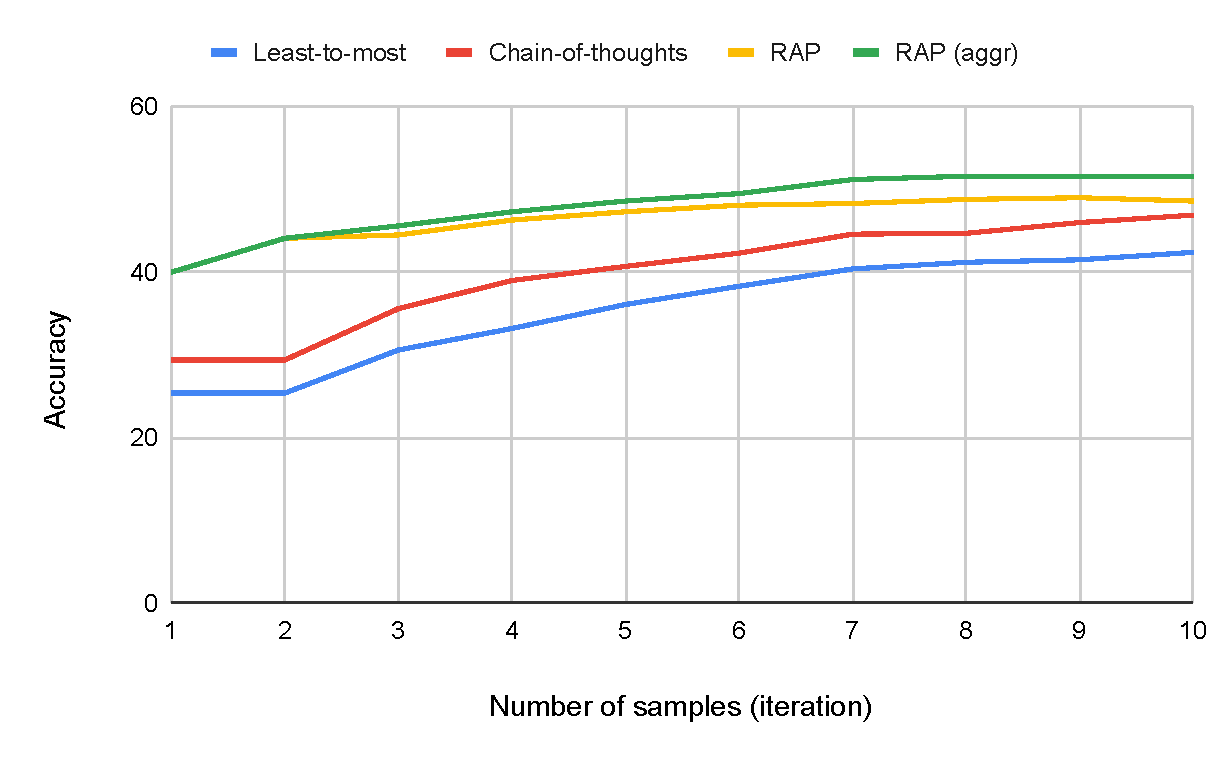
\includegraphics[width=\textwidth]{sections/chart.pdf}
%     %PLACEHOLDER \\
%     % \gy{Maybe we can put the table and figure side-by-side} It's ok to keep current format, fitting EMNLP's double-column format
%     \caption{\hsb{a figure (x-n\_samples, y-acc)}}
%     \label{fig:gsm8k-n_sample}
% \end{figure}

As a related work, Least-to-Most prompting \cite{zhou2022least} shares a similar idea to us in sub-question decomposition, but they generate sub-questions all at once. On the contrary, RAP considers each action $a_t$ based on the current state $s_t$, which enables more informed decisions.


\begin{figure}
\centering
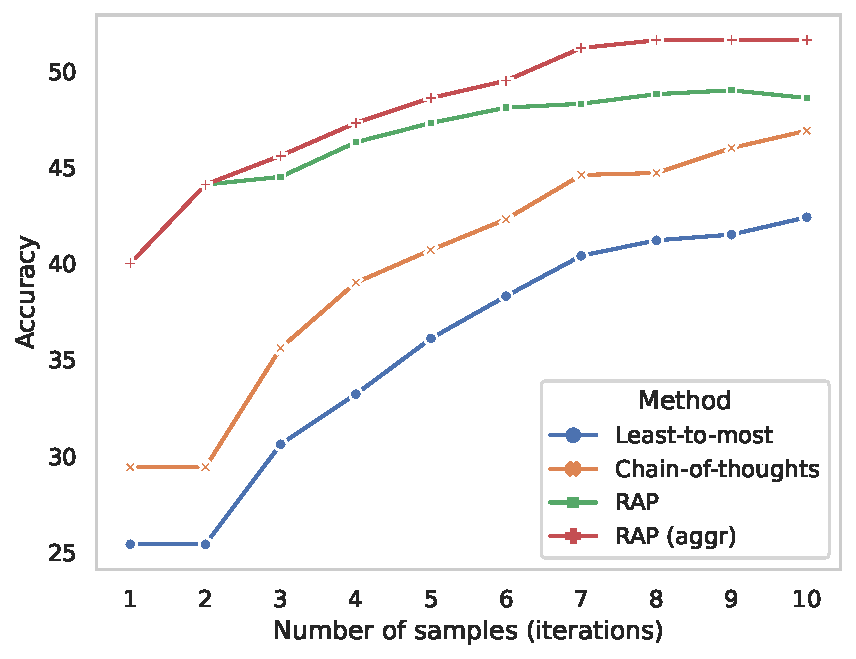
\includegraphics[width=0.8\linewidth]{sections/rap_results.pdf}
\vspace{-8pt}
\captionof{figure}{Results on GSM-8K, with different numbers of sampled paths or iterations.}
\label{fig:gsm8k-n_sample}
\vspace{-12pt}
\end{figure}




\noindent \textbf{Results.}
% \paragraph{Results.}
We evaluate our framework on GSM8k, a dataset of grade school math word problems. We also evaluate the base model with CoT prompting \cite{wei2022chain}, Least-to-Most prompting \cite{zhou2022least}, and their self-consistency \cite{wang2022self} variants, as the baselines. 
%\hzt{and self-consistency, please be complete}.
We use the same 4-shot examples demonstrations for all methods. % 10 iterations in MCTS and 10 samples in self-consistency baselines.
%\hzt{of baselines? Please be specific}.

As shown in Table \ref{tab:gsm8k}, our RAP framework answers $48.8\%$ of the problems correctly, outperforming both the Chain-of-Thought and the Least-to-Most prompting with Self-Consistency. Notably, this result is achieved when RAP only selects only one reasoning trace based on the reward.
The introduction of RAP-Aggregate further improves the accuracy by $\sim 3\%$.
We also calculate the accuracy with different numbers of iterations in MCTS and self-consistency samples in baselines, as illustrated in Figure \ref{fig:gsm8k-n_sample}.
We find that across all numbers of iterations/samples, \ours-Aggregation outperforms baselines consistently, which indicates that when only a few iterations/samples are allowed, our framework is significantly better at finding reliable reasoning paths with the guide of reward. 

\subsection{Logical Reasoning} \label{sec:logical}



\noindent \textbf{Task setup.}
% \paragraph{Task setup.}
% ProofWriter \cite{tafjord2020proofwriter}, FOLIO \cite{han2022folio}
%There exist many datasets for logical reasoning tasks, such as PrOntoQA \cite{saparov2022language}.
% In these datasets, one reasoning task typically comprises a set of facts and rules, along with a question presented a hypothesis fact to be determined true or false based solely on the given information.
A logical reasoning task (e.g. PrOntoQA \cite{saparov2022language}) typically provides a set of \emph{facts} and \emph{logical rules}, and a model is required to verify if a \emph{hypothesis fact} is true or false by applying the logical rules to the given facts, as illustrated in Figure \ref{fig:tree_examples}. These tasks not only require the correct final answer (true/false), but also a detailed proof demonstrating the result. To apply our framework, we define the \textbf{state} as a fact we are focusing on, analogous to the human's working memory~\cite{baddeley1992working} for inference. 
% \hzt{This is unclear, do you mean the pre-given set of facts, or also including the new facts derived during reasoning?}
An \textbf{action} is defined as selecting a rule from the fact set. The world model performs a one-hop reasoning step to get a new fact as the next state. The \textbf{reward} is calculated with Self-evaluation (Section~\ref{sec:reward}. Specifically, we prompt the LLM with a few examples with their labels to help it better understand the quality of reasoning steps.
% \hzt{the Method section does not use "state transition" much}.
% We also query the world model with the prompt \texttt{Is this reasoning step correct?}, \hzt{Reward is not part of world model.} and utilize the probability of the token \texttt{Yes} as the reward $r_t$.
We use the average reward of future steps to update \textbf{the $Q$ function}, the same as Equation (\ref{eq:q-avg}) for GSM8k.
% Among the logical reasoning datasets, PrOntoQA has a special characteristic in which each rule contains only one premise, resulting in a proof structured as a chain where only the new fact from the last step is required for each reasoning step.
% In such case, we can simplify our state design to be a single fact instead of a set of facts, and the state transition will involve employing the single fact and the proposed rule to perform a 1-hop reasoning and lead to the next state consisting of the new fact.
% We illustrate our world model's state and action definition in Figure \gy{figure}.


%\begin{figure}
%  \centering
%  % \vspace{-20pt}
%    \centering
%    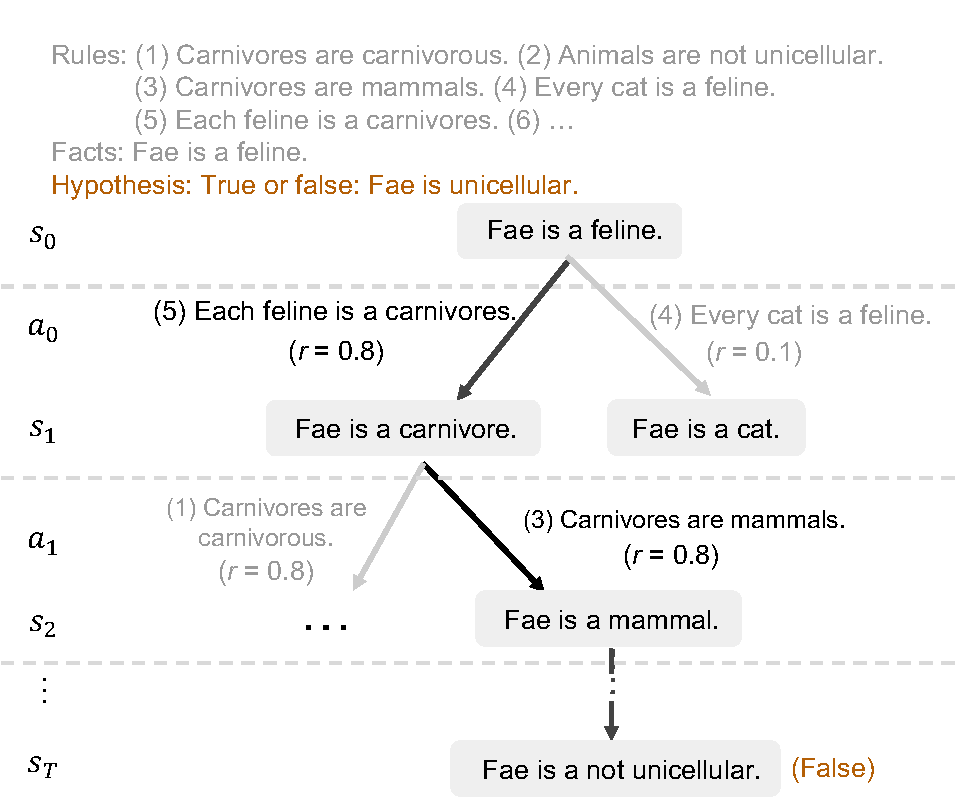
\includegraphics[scale=0.45]{sections/tree_logical.pdf}
%    \captionof{figure}{RAP planning on a PrOntoQA example.}
%    \label{fig:tree_logical}
%  \vspace{0pt}
%\end{figure}

\begin{table}
\centering
\small
\begin{tabular}{l c c}
    \toprule
    \textbf{Method} & \textbf{Pred Acc} & \textbf{Proof Acc} \\
    \midrule
    CoT & 87.8 & 64.8 \\
    CoT + SC & 89.8 & - \\
    \midrule
    RAP (Ours) & \textbf{94.2} & \textbf{78.8} \\
    \bottomrule
\end{tabular}
\vspace{-5pt}
\caption{Results on ProntoQA.}
\vspace{-15pt}
\label{tab:prontoqa}
\end{table}


\begin{table*}[ht!]
    \small
    \centering
    %\vspace{5pt}
    \begin{tabular}{c c c c c c c c c}
        \toprule
        \textbf{Setting} & \textbf{Method} & \textbf{2-step} & \textbf{4-step} & \textbf{6-step} & \textbf{8-step} & \textbf{10-step} & \textbf{12-step} & \textbf{All}\\
        \midrule
        Easy & CoT & 0.49 & 0.18 & 0.06 & 0.01 & 0.01 & 0.00 & 0.08\\
        & RAP$^{(10)}$ & 1.00 & 0.99 & 0.75 & 0.61 & 0.32& 0.32 & 0.65\\
        \midrule
        Hard & CoT & 0.22 & 0.14 & 0.02 & 0.02 & 0.00 & 0.00 & 0.05\\
        & RAP$^{(10)}$ & 0.67 & 0.76 & 0.74 & 0.48 & 0.17 & 0.09 & 0.51 \\
        \bottomrule
    \end{tabular}
    \vspace{-5pt}
    \caption{Results on the full \blocksworld with Llama-2 70B.}
    \label{tab:bw_full}
    \vspace{-15pt}
\end{table*}


\noindent \textbf{Results.}
% \paragraph{Results.}
We assess the performance of our RAP framework on PrOntoQA \cite{saparov2022language} and adopt their settings of ``true'' ontology (using real-world knowledge), ``random'' ordering of rules. We mix the examples requiring 3, 4, and 5 reasoning hops in a correct proof to prevent LLM from memorizing when to finish the reasoning. We sample 500 examples from the generation script released by \citet{saparov2022language}.
% \gy{not sure whether to mention (1) they only release the generation script, so we use that to generate 500 examples (2) intuition to mix 3, 4, 5-hop examples}
% We generate 500 examples by adhering to the dataset's ``true'' ontology, incorporating a mixture 3, 4 and 5-hop examples to discourage any potential exploitation of knowing when to finish the reasoning process
% \hzt{Cannot understand this sentence. Why do we "generate examples"? What does "adhering to the dataset's `true' ontology" mean? What does "3, 4 and 5-hop examples" mean? Also "discourage any potential exploitation of knowing when to finish the reasoning process" is hard to read}.
% We use chain-of-thought prompting \cite{wei2022chain} and its self-consistency \cite{wang2022self} variant as our baselines,
% \hzt{Self-consistency is another baseline --- We have two baselines. What we said here instead indicates we only have one baseline..}
We compare both the prediction accuracy of the final answer and the accuracy of the entire proof.
We do 20 iterations for MCTS and 20 samples for self-consistency.

As the results presented in Table \ref{tab:prontoqa}, our framework achieves a correct answer rate of 94.2\% and a proof accuracy of 78.8\%, surpassing the CoT baseline by 14\% proof accuracy and the self-consistency CoT baseline by $4.4\%$ prediction accuracy. Such substantial improvements clearly demonstrate the effectiveness of \ours in solving logical reasoning problems in PrOntoQA. Also, as the case illustrated in Figure~\ref{fig:tree_examples}, RAP can effectively recognize when a reasoning chain comes to a dead end, and propagate the signal back to earlier reasoning steps, with the planning algorithm allowing it to explore alternatives to the previous steps. The self-evaluation reward further helps RAP to recognize potential incorrect reasoning steps, encouraging the agent to avoid them in future iterations.

% Along with the self-evaluation reward, it informs the LLM of possible bad actions, and discourages further visits to this node.
% The self-evaluation helps RAP recognize the possible bad reasoning steps, discouraging further 
%\gy{why} \hzt{Does the original PrOntoQA paper report any results of other models like GPT3?}

\section{Analysis}
\subsection{Complex problems}

% Table moved to experiment.tex for positioning

To further study whether RAP can help stronger LLMs to solve more complex problems, we conduct experiments on the full Blocksworld \cite{valmeekam2023planning} dataset using a more capable LLM, Llama-2 70B \cite{touvron2023llama2}. 

The full \blocksworld \cite{valmeekam2023planning} comprises 602 test cases. We group them based on the minimum number of actions required for each test case. % The distribution of minimum numbers is visualized in Figure~\ref{fig:hist}.
Our experiments are conducted in two distinct settings: \texttt{Easy} and \texttt{Hard}. In \texttt{Easy} setting, we assume prior knowledge of the minimum number of actions for each case. Leveraging this information, we use demonstration cases that share the same minimum number of actions as the test case.
For each group of cases, we randomly select 10 cases to create a pool of demonstration cases, leaving the remaining cases as the test set. During inference, we randomly sample 4-shot demonstration cases from this pool and utilize them to formulate prompts.
% , following a similar format to the examples shown in Appendix~\ref{sec:bw_prompt}.
In the \texttt{Hard} setting, we randomly select 10 cases from the full dataset to form a demonstration pool and subsequently exclude these cases from the test set.
During inference, we randomly sample 4-shot demonstration cases from this global pool, irrespective of the minimum number of actions required for the test case.

We employ chain-of-thought prompting \cite{wei2022chain} as a baseline, and evaluate our RAP$^{(10)}$ (with 10 iterations) with an improved prompting technique (Appendix~\ref{sec:adaptive}). Our experimental results are summarized in Table~\ref{tab:bw_full}. In both the \texttt{Easy} and \texttt{Hard} settings, RAP demonstrates superior performance over CoT by a substantial margin. Notably, when the test case necessitates a larger number of steps (six or more) to solve, CoT exhibits a severe drop in success rates, whereas RAP maintains a relatively high success rate. Comparing these results with Section~\ref{sec:plan}, we additionally conclude that RAP is a general framework able to enhance the reasoning abilities of LLMs, regardless of their intrinsic capabilities.

% \begin{figure}
%     \centering
%     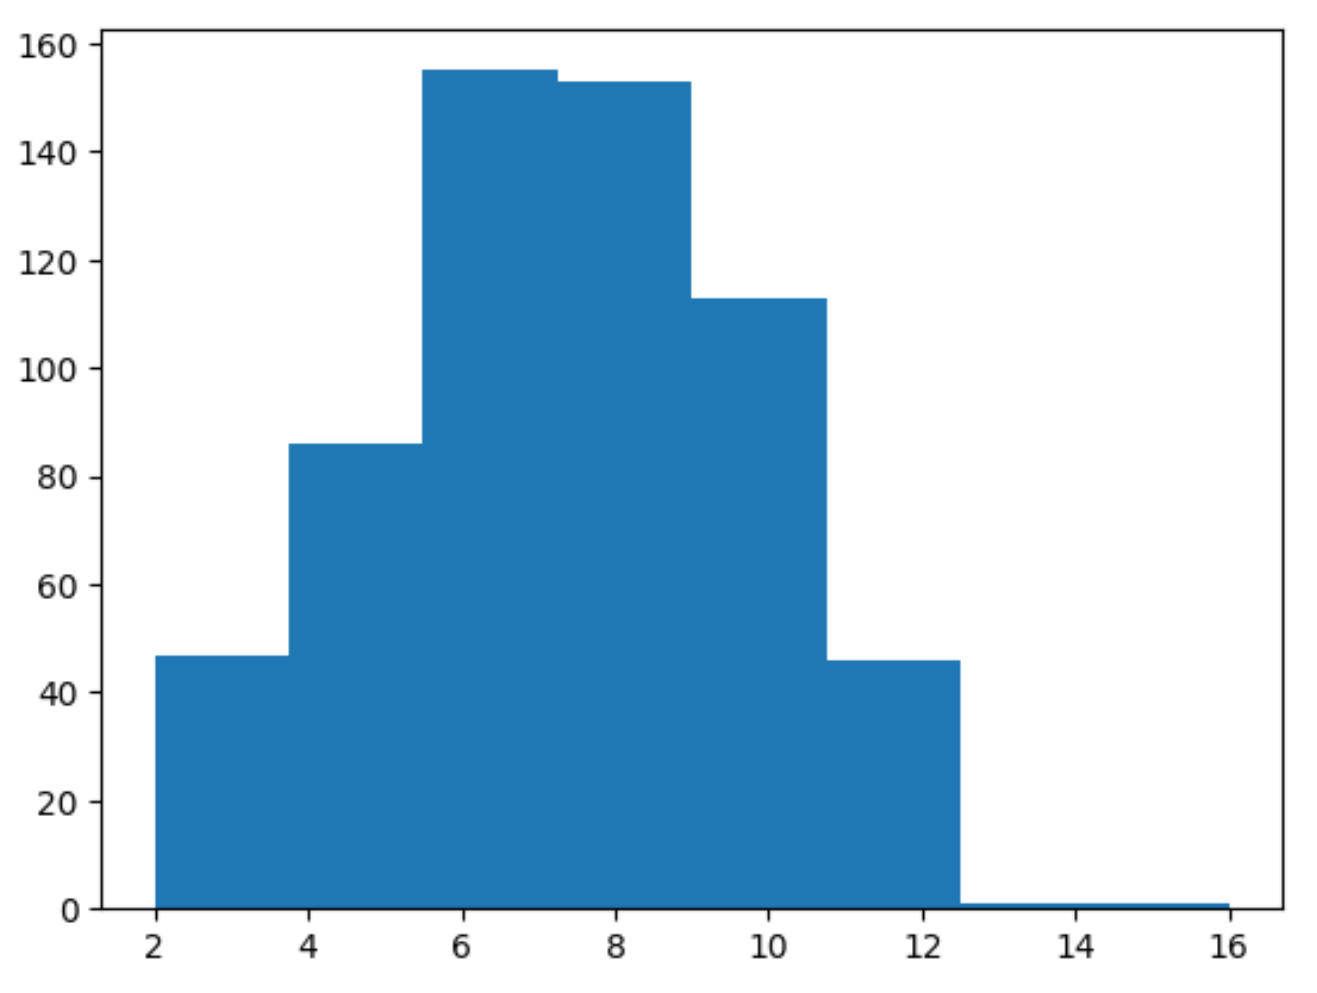
\includegraphics[width=0.9\linewidth]{sections/hist.png}
%     \caption{The statistics of minimal action number for all test cases in \blocksworld}
%     \label{fig:hist}
% \end{figure}


\subsection{Reward Choice}

\label{sec:ablation}
In our main experiments, we choose the combination of rewards in our current experiments based on heuristics and our exploratory experiments. To understand the effects of the reward choice for LLM reasoning, we supplement comprehensive experiments on rewards for plan generation (Table~\ref{tab:bw_ablation}) and math reasoning (Table~\ref{tab:gsm8k_ablation}).

Generally, the combination of multiple rewards contributes to the performance. However, the effects of a reward depends on the nature of tasks. For example, the action likelihood reward is essential for plan generation, but not very helpful to mathmatical reasoning. More discussions are in Appendix~\ref{sec:reward_appendix}.


% \vspace{-5pt}
\section{Conclusion}
% \vspace{-5pt}




In this paper, we present Reasoning via Planning (RAP), a novel LLM reasoning framework that equips LLMs with an ability to reason akin to human-like strategic planning. Our framework, which repurposes the LLM to act as both a world model and a reasoning agent, enables the LLM to simulate states of the world and anticipate action outcomes, and achieve an effective balance between exploration and exploitation via Monte-Carlo Tree Search. Extensive experiments on a variety of challenging reasoning problems demonstrate RAP's superiority over several contemporary CoT-based reasoning approaches, and even the advanced GPT-4 in certain settings. 

% RAP's flexibility in formulating rewards, states, and actions further proves its potential as a general framework for solving diverse reasoning tasks. We posit that RAP, with its innovative melding of planning and reasoning, has the potential to redefine the way we approach LLM reasoning - essentially forging a new pathway toward achieving human-level strategic thinking and planning in artificial intelligence.

\section*{Limitations}
In this work, we mainly focus on utilizing frozen LLMs, whose abilities might be bounded by the pre-training. In the future, it is worth exploring how to fine-tune LLMs to better reason and serve as a world model \cite{xiang2023language}, as well as how to combine external tools \cite{hao2023toolkengpt,schick2023toolformer} with RAP to solve more complex real-world problems.

\section*{Ethics Statement}
In this paper, we primarily focus on the applications on
plan generation, mathematical reasoning, and logical reasoning, posing no significant ethical concerns. We recognize that future research on border applications of reasoning with LLMs may pose a risk of misuse, and we recommend careful consideration of all aspects of safety before relevant techniques are applied to the real world.
%Scientific work published at EMNLP 2023 must comply with the \href{https://www.aclweb.org/portal/content/acl-code-ethics}{ACL Ethics Policy}. We encourage all authors to include an explicit ethics statement on the broader impact of the work, or other ethical considerations after the conclusion but before the references. The ethics statement will not count toward the page limit (8 pages for long, 4 pages for short papers).

% Entries for the entire Anthology, followed by custom entries
\bibliography{main}
\bibliographystyle{acl_natbib}


\appendix
\newpage



\section{MCTS Planning}
\label{sec:mcts_app}
We adapt MCTS to search for the optimal reasoning path (Algorithm~\ref{alg:mcts}). Compared with traditional applications of MCTS, we are faced with a large reasoning space, and the heavy computational cost of LLMs. Thus, we made several modifications to the classic MCTS in our implementation: (1) For open domain problems, e.g., math problems, it's impossible to enumerate all actions (subquestions), so we reduce the action space by sampling a fixed number of potential actions from LLMs, conditioned on a prompt of the current state and in-context demonstration. (2) In the selection phase, if there are actions that haven't been visited before, we estimate the Q value with lightweight local rewards, e.g., self-evaluation reward, and then select the action with UCT. This provides prior knowledge for the exploration, which is crucial given the limited iteration budgets.


\begin{algorithm*}[t]
\centering
\caption{RAP-MCTS}\label{alg:mcts}
\begin{minipage}{0.9\linewidth} 
\small
\begin{algorithmic}[1]
    \Require Initial state $s_0$, state transition probability function $p_\theta$, reward function $r_\theta$, action generator $p_\phi$, number of generated actions $d$, depth limit $L$, number of roll-outs $N$, and exploration weight $w$
    % \Statex
    \State Initialize memory of actions $A : \mathcal S \mapsto \mathcal A$, children $c : \mathcal S \times \mathcal A \mapsto \mathcal S$ 
    and rewards $r : \mathcal S \times \mathcal A \mapsto \mathbb R$ \State Initialize the state-action value function $Q : \mathcal S \times \mathcal A \mapsto \mathbb R$ and visit counter $N : \mathcal S \mapsto \mathbb N$
    \For {$n \gets 0, \dots, N - 1$}
        \State $t \gets 0$
        \While {$N(s_t) > 0$} \Comment{Selection}
            \State $N(s_t) \gets N(s_t) + 1$
            \State $a_t \gets \arg\max_{a \in A(s_t)} \left[ Q(s_t, a) + w \sqrt{\frac{\ln N(s_t)}{N(c(s_t, a))}} \right]$
            \State $r_t = r(s_t, a_t)$, $s_{t+1} \gets c(s_t, a_t)$
            \State $t \gets t + 1$
        \EndWhile
        \While {$s_t$ is not a terminal state $\wedge$ $t \leq L$}
            \For {$i \gets 1, \dots, d$} \Comment{Expansion}
                \State Sample $a_t^{(i)} \sim p_\phi(a \mid s_t)$, $s_{t+1}^{(i)} \sim p_\theta(s_t, a_t^{(i)})$, and $r_t^{(i)} \sim r_\theta(s_t, a_t^{(i)})$
                \State Update $A(s_t) \gets \{a_t^{(i)}\}_{i=1}^d$, $c(s_t, a_t^{(i)}) \gets s_{t+1}^{(i)}$, and $r(s_t, a_t) \gets r_t^{(i)}$
            \EndFor
            \State $a_{t+1} \gets \arg \max_{a \in A(s_t)} r(s_t, a_t)$ \Comment{Simulation}
            \State $r_t \gets r(s_t, a_t)$, $s_{t+1} \gets c(s_t, a_t)$
            \State $t \gets t + 1$
        \EndWhile
        \For {$t' \gets t, \dots, 0$} \Comment{Back propagation}
            \State Update $Q(s_{t'}, a_{t'})$ with $\{r_{t'}, r_{t'+1}, \dots, r_t\}$
        \EndFor
    \EndFor
\end{algorithmic}
\end{minipage}
\end{algorithm*}

\section{Experiment Settings}
\label{sec:details}
\subsection{Language Model Decoding}
We use random sampling with a temperature of 0.8. The generation is cut off at the maximum length of 2048 or a newline token.

\subsection{Computing Resources}
All of our experiments run on 4 $\times$ NVIDIA A5000 GPUs with 24GB memory.

\section{Prompt}
\label{sec:prompt}
\subsection{Plan Generation}
\label{sec:bw_prompt}
We show the prompt to calculate the action likelihood for RAP below. The same prompt is also applied in CoT baseline. \texttt{<init\_state>} and \texttt{<goals>} would be instantiated by the problem to solve.
\begin{lstlisting}[breaklines=true,breakatwhitespace=true]
I am playing with a set of blocks where I need to arrange the blocks into stacks. Here are the actions I can do

Pick up a block
Unstack a block from on top of another block
Put down a block
Stack a block on top of another block

I have the following restrictions on my actions:
I can only pick up or unstack one block at a time.
I can only pick up or unstack a block if my hand is empty.
I can only pick up a block if the block is on the table and the block is clear. A block is clear if the block has no other blocks on top of it and if the block is not picked up.
I can only unstack a block from on top of another block if the block I am unstacking was really on top of the other block.
I can only unstack a block from on top of another block if the block I am unstacking is clear.
Once I pick up or unstack a block, I am holding the block.
I can only put down a block that I am holding.
I can only stack a block on top of another block if I am holding the block being stacked.
I can only stack a block on top of another block if the block onto which I am stacking the block is clear.
Once I put down or stack a block, my hand becomes empty.

[STATEMENT]
As initial conditions I have that, the red block is clear, the yellow block is clear, the hand is empty, the red block is on top of the blue block, the yellow block is on top of the orange block, the blue block is on the table and the orange block is on the table.
My goal is to have that the orange block is on top of the red block.

My plan is as follows:

[PLAN]
unstack the yellow block from on top of the orange block
put down the yellow block
pick up the orange block
stack the orange block on top of the red block
[PLAN END]

[STATEMENT]
As initial conditions I have that, the orange block is clear, the yellow block is clear, the hand is empty, the blue block is on top of the red block, the orange block is on top of the blue block, the red block is on the table and the yellow block is on the table.
My goal is to have that the blue block is on top of the red block and the yellow block is on top of the orange block.

My plan is as follows:

[PLAN]
pick up the yellow block
stack the yellow block on top of the orange block
[PLAN END]

[STATEMENT]
As initial conditions I have that, the red block is clear, the blue block is clear, the orange block is clear, the hand is empty, the blue block is on top of the yellow block, the red block is on the table, the orange block is on the table and the yellow block is on the table.
My goal is to have that the blue block is on top of the orange block and the yellow block is on top of the red block.

My plan is as follows:

[PLAN]
unstack the blue block from on top of the yellow block
stack the blue block on top of the orange block
pick up the yellow block
stack the yellow block on top of the red block
[PLAN END]

[STATEMENT]
As initial conditions I have that, the red block is clear, the blue block is clear, the yellow block is clear, the hand is empty, the yellow block is on top of the orange block, the red block is on the table, the blue block is on the table and the orange block is on the table.
My goal is to have that the orange block is on top of the blue block and the yellow block is on top of the red block.

My plan is as follows:

[PLAN]
unstack the yellow block from on top of the orange block
stack the yellow block on top of the red block
pick up the orange block
stack the orange block on top of the blue block
[PLAN END]

[STATEMENT]
As initial conditions I have that, <initial_state>
My goal is to have that <goals>.

My plan is as follows:

[PLAN]
\end{lstlisting}

For the next state prediction with the world model, we apply the prompts conditioned on the last action. Here we show the prompt to update the state after a ``\texttt{pick up}'' action as an example. Again, \texttt{<state>} and \texttt{<action>} would be instantiated with the current state and action.

\begin{lstlisting}[breaklines=true,breakatwhitespace=true]
I am playing with a set of blocks where I need to arrange the blocks into stacks. Here are the actions I can do 

Pick up a block 
Unstack a block from on top of another block 
Put down a block 
Stack a block on top of another block 

I have the following restrictions on my actions:
I can only pick up or unstack one block at a time. 
I can only pick up or unstack a block if my hand is empty. 
I can only pick up a block if the block is on the table and the block is clear. A block is clear if the block has no other blocks on top of it and if the block is not picked up. 
I can only unstack a block from on top of another block if the block I am unstacking was really on top of the other block. 
I can only unstack a block from on top of another block if the block I am unstacking is clear. Once I pick up or unstack a block, I am holding the block. 
I can only put down a block that I am holding. 
I can only stack a block on top of another block if I am holding the block being stacked. 
I can only stack a block on top of another block if the block onto which I am stacking the block is clear. Once I put down or stack a block, my hand becomes empty.

After being given an initial state and an action, give the new state after performing the action.

[SCENARIO 1]
[STATE 0] I have that, the white block is clear, the cyan block is clear, the brown block is clear, the hand is empty, the white block is on top of the purple block, the purple block is on the table, the cyan block is on the table and the brown block is on the table.
[ACTION] Pick up the brown block.
[CHANGE] The hand was empty and is now holding the brown block, the brown block was on the table and is now in the hand, and the brown block is no longer clear.
[STATE 1] I have that, the white block is clear, the cyan block is clear, the brown block is in the hand, the hand is holding the brown block, the white block is on top of the purple block, the purple block is on the table and the cyan block is on the table.

[SCENARIO 2]
[STATE 0] I have that, the purple block is clear, the cyan block is clear, the white block is clear, the hand is empty, the white block is on top of the brown block, the purple block is on the table, the cyan block is on the table and the brown block is on the table.
[ACTION] Pick up the cyan block.
[CHANGE] The hand was empty and is now holding the cyan block, the cyan block was on the table and is now in the hand, and the cyan block is no longer clear.
[STATE 1] I have that, the cyan block is in the hand, the white block is clear, the purple block is clear, the hand is holding the cyan block, the white block is on top of the brown block, the purple block is on the table and the brown block is on the table.

[SCENARIO 3]
[STATE 0] <state>
[ACTION] <action>
[CHANGE]
\end{lstlisting}

\subsection{Math Reasoning}
We show the prompt of RAP for math reasoning as below. The prompt is used for both action proposal and next state prediction. After instantiate \texttt{<question>}, we append a prefix \texttt{Question 5.1} to the prompt, so that we can sample the first action with the LLM. The future actions are sampled similarly, except that all previous sub-questions and sub-answers need to be appended to the prompt, following the formats of in-context demonstration. The next state prediction, i.e., answering the sub-question, works in the same way.

\begin{lstlisting}[breaklines=true,breakatwhitespace=true]
Given a question, please decompose it into sub-questions. For each sub-question, please answer it in a complete sentence, ending with "The answer is". When the original question is answerable, please start the subquestion with "Now we can answer the question: ".

Question 1: Four years ago, Kody was only half as old as Mohamed. If Mohamed is currently twice as 30 years old, how old is Kody?
Question 1.1: How old is Mohamed?
Answer 1.1: He is currently 30 * 2 = 60 years old. The answer is 60.
Question 1.2: How old was Mohamed four years ago?
Answer 1.2: Four years ago, he must have been 60 - 4 = 56 years old. The answer is 56.
Question 1.3: How old was Kody four years ago?
Answer 1.3: Kody was half as old as Mohamed four years ago. Thus, Kody was 56 / 2 = 28 years old. The answer is 28.
Question 1.4: Now we can answer the question: How old is Kody?
Answer 1.4: She is currently 28 + 4 = 32 years old. The answer is 32.

Question 2: On a moonless night, three fireflies danced in the evening breeze. They were joined by four less than a dozen more fireflies before two of the fireflies flew away. How many fireflies remained?
Question 2.1: How many fireflies joined?
Answer 2.1: The fireflies were joined by four less than a dozen more fireflies, which are 12 - 4 = 8 fireflies. The answer is 8.
Question 2.2: Now we can answer the question: How many fireflies remained?
Answer 2.2: Three fireflies were dancing originally. They were joined by 8 fireflies before two of them flew away. So there were 3 + 8 - 2 = 9 remaining. The answer is 9.

Question 3: Ali has four $10 bills and six $20 bills that he saved after working for Mr. James on his farm. Ali gives her sister half of the total money he has and uses 3/5 of the remaining amount of money to buy dinner. Calculate the amount of money he has after buying the dinner.
Question 3.1: How much money does Ali have in total?
Answer 3.1: Ali has four $10 bills and six $20 bills. So he has 4 * 10 + 6 * 20 = 160 dollars. The answer is 160.
Question 3.2: How much money does Ali give to his sister?
Answer 3.2: Ali gives half of the total money he has to his sister. So he gives 160 / 2 = 80 dollars to his sister. The answer is 80.
Question 3.3: How much money does Ali have after giving his sister the money?
Answer 3.3: After giving his sister the money, Ali has 160 - 80 = 80 dollars left. The answer is 80.
Question 3.4: How much money does Ali use to buy dinner?
Answer 3.4: Ali uses 3/5 of the remaining amount of money to buy dinner. So he uses 80 * 3/5 = 48 dollars to buy dinner. The answer is 48.
Question 3.5: Now we can answer the question: How much money does Ali have after buying the dinner?
Answer 3.5: After buying the dinner, Ali has 80 - 48 = 32 dollars left. The answer is 32.

Question 4: A car is driving through a tunnel with many turns. After a while, the car must travel through a ring that requires a total of 4 right-hand turns. After the 1st turn, it travels 5 meters. After the 2nd turn, it travels 8 meters. After the 3rd turn, it travels a little further and at the 4th turn, it immediately exits the tunnel. If the car has driven a total of 23 meters around the ring, how far did it have to travel after the 3rd turn?
Question 4.1: How far did the car travel except for the 3rd turn?
Answer 4.1: It travels 5 meters after the 1st, 8 meters after the 2nd, and 0 meters after the 4th turn. It's a total of 5 + 8 + 0 = 13 meters. The answer is 13.
Question 4.2: Now we can answer the question: How far did the car have to travel after the 3rd turn?
Answer 4.2: The car has driven a total of 23 meters around the ring. It travels 13 meters except for the 3rd turn. So it has to travel 23 - 13 = 10 meters after the 3rd turn. The answer is 10.

Question 5: <question>
\end{lstlisting}

\subsection{Logical Reasoning}
We show the prompt for action proposal, action likelihood calculation, and next state prediction. \texttt{<fact>} and \texttt{<query>} would be instantiated with the problem.
\begin{lstlisting}[breaklines=true,breakatwhitespace=true]
Given a list of facts, and a current claim, output one possible fact as the next step. Be sure to copy the exact sentences in the facts. Do not change any wording. Do not create your own words.

Facts 1: Each lepidopteran is an insect. Each arthropod is a protostome. Every animal is multicellular. Protostomes are invertebrates. Each whale is bony. Each painted lady is a butterfly. Invertebrates are animals. Butterflies are lepidopterans. Each insect is six-legged. Every insect is an arthropod. Arthropods are not bony.
Query 1: True or false: Sally is not bony.
Claim 1.1: Sally is an insect.
Next 1.1: Each insect is six-legged.
Claim 1.2: Sally is a butterfly.
Next 1.2: Butterflies are lepidopterans.
Claim 1.3: Sally is a lepidopteran.
Next 1.3: Each lepidopteran is an insect.
Claim 1.4: Sally is not bony.
Next 1.4: Finish.
Claim 1.5: Sally is an arthropod.
Next 1.5: Arthropods are not bony.
Claim 1.6: Sally is a painted lady.
Next 1.6: Each painted lady is a butterfly.

Facts 2: Prime numbers are natural numbers. Every Mersenne prime is not composite. Imaginary numbers are not real. Every real number is a number. Natural numbers are integers. Every real number is real. Every Mersenne prime is a prime number. Natural numbers are positive. Prime numbers are not composite. Integers are real numbers.
Query 2: True or false: 127 is not real.
Claim 2.1: 127 is real.
Next 2.1: Finish.
Claim 2.1: 127 is a natural number.
Next 2.1: Natural numbers are integers.
Claim 2.2: 127 is a prime number.
Next 2.2: Prime numbers are natural numbers.
Claim 2.3: 127 is a real number.
Next 2.3: Every real number is real.
Claim 2.4: 127 is a Mersenne prime.
Next 2.4: Every Mersenne prime is a prime number.
Claim 2.5: 127 is an integer.
Next 2.5: Integers are real numbers.

Facts 3: Lepidopterans are insects. Every animal is multicellular. Each insect is an arthropod. Each invertebrate is an animal. Insects are six-legged. Arthropods are small. Arthropods are invertebrates. Each butterfly is a lepidopteran. Whales are not small.
Query 3: True or false: Polly is not small.
Claim 3.1: Polly is an arthropod.
Next 3.1: Arthropods are small.
Claim 3.2: Polly is an insect.
Next 3.2: Each insect is an arthropod.
Claim 3.3: Polly is small.
Next 3.3: Finish.
Claim 3.4: Polly is a lepidopteran.
Next 3.4: Lepidopterans are insects.

Facts 4: Every cat is a feline. Mammals are vertebrates. Bilaterians are animals. Vertebrates are chordates. Carnivores are mammals. Mammals are not cold-blooded. Each chordate is a bilaterian. Every feline is a carnivore. Snakes are cold-blooded. Animals are not unicellular. Every carnivore is not herbivorous.
Query 4: True or false: Fae is not cold-blooded.
Claim 4.1: Fae is a feline.
Next 4.1: Every feline is a carnivore.
Claim 4.2: Fae is not cold-blooded.
Next 4.2: Finish.
Claim 4.2: Fae is a mammal.
Next 4.2: Mammals are not cold-blooded.
Claim 4.3: Fae is a cat.
Next 4.3: Every cat is a feline.
Claim 4.4: Fae is a carnivore.
Next 4.4: Carnivores are mammals.

Facts 5: Prime numbers are prime. Real numbers are numbers. Every integer is a real number. Real numbers are not imaginary. Mersenne primes are prime numbers. Complex numbers are imaginary. Each prime number is a natural number. Natural numbers are positive. Each Mersenne prime is prime. Each natural number is an integer.
Query 5: True or false: 7 is imaginary.
Claim 5.1: 7 is not imaginary.
Next 5.1: Finish.
Claim 5.1: 7 is a natural number.
Next 5.1: Each natural number is an integer.
Claim 5.2: 7 is a prime number.
Next 5.2: Each prime number is a natural number.
Claim 5.3: 7 is a real number.
Next 5.3: Real numbers are not imaginary.
Claim 5.4: 7 is an integer.
Next 5.4: Every integer is a real number.

Facts 6: Spiders are not six-legged. Insects are six-legged. Insects are arthropods. Every animal is not unicellular. Invertebrates are animals. Lepidopterans are insects. Every arthropod is segmented. Arthropods are invertebrates. Every butterfly is a lepidopteran. Stella is a butterfly.
Query 6: True or false: Stella is six-legged.
Claim 6.1: Stella is an insect.
Next 6.1: Insects are six-legged.
Claim 6.2: Stella is a lepidopteran.
Next 6.2: Lepidopterans are insects.
Claim 6.3: Stella is a butterfly.
Next 6.3: Every butterfly is a lepidopteran.
Claim 6.4: Stella is six-legged.
Next 6.4: Finish.

Facts 7: <fact>
Query 7: <query>
\end{lstlisting}

% \section{Extended experiments on Blocksworld}
% \label{sec:bw_appendix_full}
% In this section, we present an in-depth exploration of the reasoning abilities of advanced LLMs on more challenging problems. We extend our experiments to the full Blocksworld \cite{valmeekam2023planning} using the more potent Llama-2 70B \cite{touvron2023llama}. 

% \noindent \textbf{Experiment setting.} The full dataset we use is sourced from \citet{valmeekam2023planning}, comprising 602 test cases. We group them based on the minimum number of actions required for each test case. The distribution of minimum numbers is visualized in Figure~\ref{fig:hist}.

% Our experiments are conducted in two distinct settings: \texttt{Easy} and \texttt{Hard}. In \texttt{Easy} setting, we assume prior knowledge of the minimum number of actions for each case. Leveraging this information, we use demonstration cases that share the same minimum number of actions as the test case.
% For each group of cases, we randomly select 10 cases to create a pool of demonstration cases, leaving the remaining cases as the test set. During inference, we randomly sample 4-shot demonstration cases from this pool and utilize them to formulate prompts, following a similar format to the examples shown in Appendix~\ref{sec:bw_prompt}.
% In the \texttt{Hard} setting, we randomly select 10 cases from the full dataset to form a demonstration pool and subsequently exclude these cases from the test set.
% During inference, we randomly sample 4-shot demonstration cases from this global pool, irrespective of the minimum number of actions required for the test case.

% \begin{table*}[t!]
%     \small
%     \centering
%     %\vspace{5pt}
%     \begin{tabular}{c c c c c c c c c}
%         \toprule
%         \textbf{Setting} & \textbf{Method} & \textbf{2-step} & \textbf{4-step} & \textbf{6-step} & \textbf{8-step} & \textbf{10-step} & \textbf{12-step} & \textbf{All}\\
%         \midrule
%         Easy & CoT & 0.49 & 0.18 & 0.06 & 0.01 & 0.01 & 0.00 & 0.08\\
%         & RAP$^{(10)}$ & 1.00 & 0.99 & 0.75 & 0.61 & 0.32& 0.32 & 0.65\\
%         \midrule
%         Hard & CoT & 0.22 & 0.14 & 0.02 & 0.02 & 0.00 & 0.00 & 0.05\\
%         & RAP$^{(10)}$ & 0.67 & 0.76 & 0.74 & 0.48 & 0.17 & 0.09 & 0.51 \\
%         \bottomrule
%     \end{tabular}
%     % \vspace{4pt}
%     \caption{Results on the full \blocksworld with Llama-2 70B.}
%     \label{tab:bw_full}
%     \vspace{-5pt}
% \end{table*}

% \noindent \textbf{Methods.} For our experimentation, we employ chain-of-thought prompting \cite{wei2022chain} as a baseline, and evaluate our RAP$^{(10)}$ (with 10 iterations) with an adaptive prompting technique. Through our preliminary experiments, we observed that the performance of LLMs is impacted by the discrepancy in difficulty between demonstration cases and the test cases. In the case of RAP, when a new state is predicted, we reformulate the remaining task as a new test case, initialized with the predicted new state. This new test case would require a smaller minimum number of actions, leading to a disparity in the distribution of the demonstration cases and the new cases. To mitigate this issue, we pre-compute the intermediate states of the demonstration cases beforehand. During inference, we truncate the trace from the beginning for each new state in an iteration, which reduces the minimum action number of the demonstration cases as the search tree deepens. This technique significantly enhances the performance of RAP, especially for more intricate problems, which are more susceptible to distribution mismatches.

% \noindent \textbf{Results.} Our experimental results are summarized in Table~\ref{tab:bw_full}. In both the \texttt{Easy} and \texttt{Hard} settings, RAP demonstrates superior performance over CoT by a substantial margin. Notably, when the test case necessitates a high number of steps (six or more) to solve, CoT exhibits a severe drop in success rates, whereas RAP maintains a relatively high success rate. When comparing this results with Section~\ref{sec:experiments}, we can also conclude that, RAP is a general framework able to enhance the reasoning abilities of LLMs, regardless of their intrinsic capabilities.

% \begin{figure}
%     \centering
%     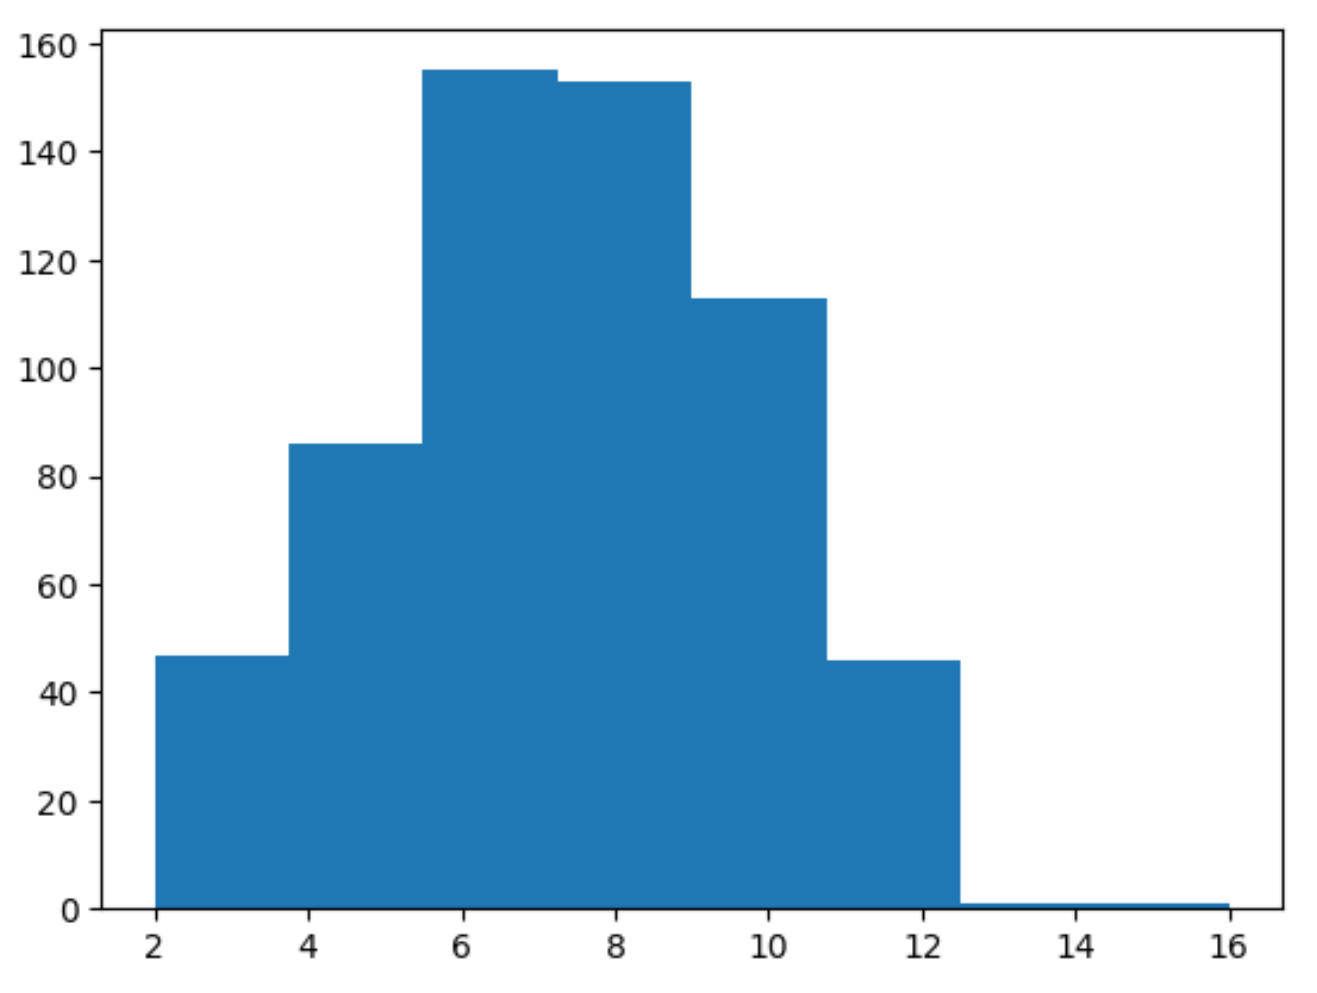
\includegraphics[width=0.9\linewidth]{sections/hist.png}
%     \caption{The statistics of minimal action number for all test cases in \blocksworld}
%     \label{fig:hist}
% \end{figure}


\section{Related work: world model and planning}
\label{sec:related_planning}
Recent years have witnessed successful applications of planning algorithms~\cite{sekar2020planning}, such as AlphaZero~\cite{silver2017mastering}, and MuZero~\cite{schrittwieser2020mastering}. These algorithms are typically based on tree-structured search and are designed to effectively maintain the balance of exploration and exploitation. Knowledge of transition dynamics is the prerequisite for planning, and recent research on model-based reinforcement learning propose to learn a world model (or dynamics model) to plan or assist policy learning. To improve sample efficiency, previous research attempts to learn a world model from offline trajectories, and directly learn a policy within the world model \cite{ha2018recurrent, ha2018world}. With latent imagination in a world model, RL agents can be trained to solve long-horizon tasks~\cite{hafner2019dream, hafner2020mastering}. Besides, the world model is also shown to be helpful to physical robot learning~\cite{wu2023daydreamer}. In this paper, we use LLMs as world models and apply a planning algorithm to search for a reasoning path. This is similar in spirit to model predictive control \cite{camacho2013model}. Compared with previous works, our framework uses general LLMs as the world model and can be adapted to a wide range of open-domain reasoning tasks. \citet{xiang2023language} propose to train LLMs wih a external world model to gain embodied experience, while RAP focuses on the inference stage and is compatible with any training methods.

\section{Adaptive Prompting}
\label{sec:adaptive}
Through our preliminary experiments, we observed that the performance of LLMs is impacted by the discrepancy in difficulty between demonstration cases and the test cases. In the case of RAP, when a new state is predicted, we reformulate the remaining task as a new test case, initialized with the predicted new state. This new test case would require a smaller minimum number of actions, leading to a disparity in the distribution of the demonstration cases and the new cases. To mitigate this issue, we pre-compute the intermediate states of the demonstration cases beforehand. During inference, we truncate the trace from the beginning for each new state in an iteration, which reduces the minimum action number of the demonstration cases as the search tree deepens. This technique significantly enhances the performance of RAP, especially for more intricate problems, which are more susceptible to distribution mismatches.

\section{Reward Choice}
\label{sec:reward_appendix}
\begin{table}[t]
    \centering
    \caption{Ablation study on Blocksworld. $R_1$ is action likelihood reward, $R_2$ is task-specific reward, and $R_3$ is self-evaluation reward.}
    % \vspace{5pt}
    \begin{tabular}{c|c|c|c}
    \toprule
        $R_1$ & $R_2$ & $R_3$ & \thead{Success} \\
        \midrule
        \cmark & \cmark & \xmark & 0.88\\
        \cmark & \cmark & \cmark & 0.91\\
        \cmark & \xmark & \xmark & 0.46\\
        \xmark & \cmark & \xmark & 0.21\\
        \xmark & \xmark & \cmark & 0.14\\
        \xmark & \xmark & \xmark & 0.02\\
    \bottomrule
    \end{tabular}
    \vspace{-5pt}
    \label{tab:bw_ablation}
\end{table}
\begin{table}[t]
  % \hspace{0.5cm}
    \centering
    \caption{Ablation study on GSM8k (first 300 examples). $R_1$ is state transition confidence reward, $R_2$ is action likelihood reward, and $R_3$ is self-evaluation reward.}
    \vspace{5pt}
    \begin{tabular}{c|c|c|c|c|c}
    \toprule
        $R_1$ & $R_2$ & $R_3$ & RAP$^{(1)}$ & RAP$^{(10)}$ & +aggr\\
        \midrule
        \cmark & \xmark & \cmark & 0.410 & 0.450 & 0.503\\
        \cmark & \xmark & \xmark & 0.350 & 0.447 & 0.490 \\
        \cmark & \cmark & \xmark & 0.373 & 0.423 & 0.443\\
         \bottomrule
    \end{tabular}
    \vspace{-5pt}
    \label{tab:gsm8k_ablation}
\end{table}
\noindent \textbf{Results.} We conduct comprehensive experiments on rewards for plan generation (Table~\ref{tab:bw_ablation}) and math reasoning (Table~\ref{tab:gsm8k_ablation}). Note that, in both tables, the first row indicates the setting we use in the main experiments. As shown in Table~\ref{tab:bw_ablation}, the combination of action likelihood and task-specific reward (row 1) can significantly outperform the single reward baselines (row 3, 4, 5). Interestingly, adding the self-evaluation reward can further improve the performance slightly (row 2). Furthermore, as the results on the first 300 samples of GSM8k shown in Table~\ref{tab:gsm8k_ablation}, we can see adding either action likelihood (row 3) or self-evaluation (row 1) on top of confidence reward (row 2) can boost the RAP performance of only using confidence reward (row 1) with one iteration, but action likelihood reward downgrades the accuracy with more iterations. The self-evaluation reward leads to the best performance overall. This indicates the importance of self-evaluation reward in guiding reasoning as an effective and computationally efficient prior to exploration.

\noindent\textbf{Self-evaluation and action likelihood.}
The rewards of self-evaluation and action likelihood are of particular interest, as they can be applied to a wide range of reasoning tasks. Generally, the best usage and combination with other rewards require empirical design and understanding of the task nature, and their effectiveness can vary significantly across different tasks. Here, we provide some intuitions behind the reward choices:

(a) For the problems in which one reasoning step is short and structured, the action likelihood can be very indicative. Otherwise, it may be disturbed by unimportant tokens and become unreliable. For instance, a single step within the Blocksworld domain typically adheres to specific patterns (e.g., \textsc{pick/put/stack} a block…), rendering the action likelihood indicative. However, in the math domain, a reasoning step is expressed in natural language sentences, allowing for greater freedom and potentially introducing noise.

(b) For the problems where it’s easier to recognize some errors afterward than avoid them during generation, self-evaluation emerges as a helpful mechanism for enhancing reasoning accuracy. In mathematical reasoning, LLMs may struggle to generate a correct reasoning step in the first place, but the detection of calculation or logic errors is more feasible. In Blocksworlds, however, assessing the quality of a candidate action is not straightforward and still requires multi-step reasoning. This characteristic diminishes the accuracy of the self-evaluation reward, making it less helpful especially given that likelihood already provides a good intuition for search.


\end{document}
